% !TeX spellcheck = en_US
% Dirty hack to disable recompiling the bibliography every time, reducing compilation times. Comment out with another % to re-compile bibliography.
% !TeX TXS-program:recompile-bibliography = donothing

% Use biber as bibliography tool
% !TeX TXS-program:bibliography = txs:///biber

\documentclass[a4paper]{scrreprt}

\usepackage[draft]{graphicx}
\usepackage{xargs}                      % Use more than one optional parameter in a new commands
\usepackage[pdftex,dvipsnames]{xcolor}  % Coloured text etc.
\usepackage[colorinlistoftodos,prependcaption,textsize=tiny]{todonotes}
\newcommandx{\error}[2][1=]{\todo[linecolor=red,backgroundcolor=red!25,bordercolor=red,#1]{#2}}
\newcommandx{\unsure}[2][1=]{\todo[linecolor=orange,backgroundcolor=orange!25,bordercolor=orange,#1]{#2}}
\newcommandx{\change}[2][1=]{\todo[linecolor=blue,backgroundcolor=blue!25,bordercolor=blue,#1]{#2}}
\newcommandx{\info}[2][1=]{\todo[linecolor=OliveGreen,backgroundcolor=OliveGreen!25,bordercolor=OliveGreen,#1]{#2}}
\newcommandx{\improvement}[2][1=]{\todo[linecolor=Plum,backgroundcolor=Plum!25,bordercolor=Plum,#1]{#2}}
\newcommandx{\thiswillnotshow}[2][1=]{\todo[disable,#1]{#2}}


\usepackage{amsfonts} 
\usepackage{amsmath}
\usepackage{amsthm} %Proof Environment
\usepackage{amssymb}
\usepackage{marvosym}
\usepackage{stmaryrd} %\lightning
\usepackage{latexsym} %\leadsto

\usepackage[utf8]{inputenc}
\usepackage[T1]{fontenc}
\usepackage[english]{babel} 

\usepackage{pdfpages} % include pdf pages
\usepackage{hyperref}
\usepackage{graphicx}

\usepackage{enumitem}
\usepackage{multicol}
\usepackage{chngcntr}

\usepackage{xifthen}

\usepackage{listings} % source listings
\usepackage{xcolor} % defining own colors: \color

\usepackage{dsfont} % \1 for identity functions

\usepackage{etoolbox}

% custom math commands:

% column vectors
\newcount\xveccount
\renewcommand*\vec[1]{
	\global\xveccount#1
	\begin{pmatrix}
		\vecnext
	}
	\def\vecnext#1{
		#1
		\global\advance\xveccount-1
		\ifnum\xveccount>0
		\\
		\expandafter\vecnext
		\else
	\end{pmatrix}
	\fi
}  
\newcommand{\vectwo}[3][0pt]{\begin{pmatrix}#2\\[#1] #3\end{pmatrix}}
\newcommand{\vecthree}[4][0pt]{\begin{pmatrix}#2\\[#1] #3\\[#1] #4\end{pmatrix}}
\newcommand{\vecfour}[5][0pt]{\begin{pmatrix}#2\\[#1] #3\\[#1] #4\\[#1] #5\end{pmatrix}}
\newcommand{\vecfive}[6][0pt]{\begin{pmatrix}#2\\[#1] #3\\[#1] #4\\[#1] #5\\[#1] #6\end{pmatrix}}

% * as multiplication dot
\mathcode`\*="8000
{\catcode`\*\active\gdef*{\cdot}}

% common number set symbols
\newcommand{\N}{\mathbb{N}}
\newcommand{\Z}{\mathbb{Z}}
\newcommand{\Q}{\mathbb{Q}}
\newcommand{\R}{\mathbb{R}}
\newcommand{\C}{\mathbb{C}}

% useful mathematical operators
\DeclareMathOperator{\Pot}{\mathcal{P}}
\DeclareMathOperator{\BigO}{\mathcal{O}}
\DeclareMathOperator{\inv}{^{-1}}
\renewcommand{\Re}[1]{\text{Re}\left( #1 \right)}
\renewcommand{\Im}[1]{\text{Im}\left( #1 \right)}
\newcommand{\abs}[1]{\left| #1 \right|}
\DeclareMathOperator{\vspan}{\text{span}}
\newcommand{\setspan}[1]{\vspan\left(\left\{#1\right\}\right)}
\DeclareMathOperator{\rang}{\text{rang}}
\newcommand{\integral}[4]{\int_{#1}^{#2} #3 \, d#4}
\newcommand{\lintegral}[3]{\int_{#1} #2 \, d#3}
\newcommand{\comp}{^\complement}
\newcommand{\ra}{\rightarrow}
\newcommand{\lra}{\Leftrightarrow} % equivalence arrow
\newcommand{\1}[1][]{\mathds{1}\ifthenelse{\isempty{#1}}{}{_{#1}}}
\newcommand{\dummydot}{\,\cdot\,}
\DeclareMathOperator{\im}{\text{im}}
\newcommand{\innerprod}[2]{\left\langle #1, #2 \right\rangle}
\DeclareMathOperator{\supp}{supp}
\newcommand{\transposed}{^{T}}
\DeclareMathOperator{\argmax}{argmax}
\DeclareMathOperator{\argmin}{argmin}
\newcommand{\colonlra}{\mathrel{\vcentcolon\Leftrightarrow}} % properly typeset :<=>

% switch-case structure
\newcommand{\ifequals}[4]{\ifthenelse{\equal{#1}{#2}}{#3}{#4}}
\newcommand{\case}{} % Dummy, so \renewcommand has something to overwrite...
\newenvironment{switch}[1]{\renewcommand{\case}[3]{\ifequals{#1}{##1}{##2}{##3}}}{} %Usage: \begin{switch}{value}, \case{value}{then}{else}

% shortcut for inline pmatrix
\newcommand{\pmat}[1]{\begin{pmatrix}#1\end{pmatrix}}

% brutally enforce centering the contents
\newcommand{\centerbrutally}[1]
{
	\centerline{
		\begin{minipage}{\linewidth}
			#1
	\end{minipage}}
}

\definecolor{verylightgray}{gray}{0.97}
\definecolor{purple}{RGB}{127,0,116} % used for keyword coloring in source code listings
\definecolor{brickred}{rgb}{0.56, 0.175, 0.231} % used for string coloring in source code listing

% norm ||x||
\newcommand{\norm}[1]{\left\lVert#1\right\rVert}

% centered inline graphics
\newcommand{\includegraphicsinline}[2][]{\begingroup\setbox0=\hbox{\includegraphics[#1]{#2}}\parbox{\wd0}{\box0}\endgroup}

% tilde in lstlisting
\lstset{literate=%
    {~}{{\textasciitilde}}1
}

% shortcuts: for limits/series going to infinity
\newcommand{\liminfty}[1]{\lim\limits_{#1 \rightarrow \infty}}
\newcommand{\ser}[1]{\sum\limits_{\ifthenelse{\isin{=}{#1}}{#1}{#1=1}}^{\infty}}
\newcommand{\toinfty}[1]{\xrightarrow{\;#1 \to \infty\;}}

% shortcut for multiple cases in math formulas: '"1", falls "2", "3", falls "4"' (bzw. 'sonst', falls leer)
\newcommand{\twocases}[4]
{
    \begin{cases}
        #1, &\text{if } #2 \\
        #3, &\ifthenelse{\isempty{#4}}{\text{else}}{\text{if } #4}
    \end{cases}
}

% shortcut for parentheses and sets
\newcommand{\pars}[1]{\left(#1\right)}
\newcommand{\bigpars}[1]{\bigl(#1\bigr)}
\newcommand{\biggpars}[1]{\biggl(#1\biggr)}
\newcommand{\set}[1]{\{#1\}}
\newcommand{\bigset}[1]{\bigl\{#1\bigr\}}
\newcommand{\biggset}[1]{\biggl\{#1\biggr\}}
\newcommand{\bigmid}{\bigm\vert}
\newcommand{\biggmid}{\biggm\vert}

\newenvironment{correction}[1]{\color{red}\textbf{\underline{#1}}\\}{\ignorespacesafterend}

\makeatletter
\patchcmd{\upbracefill}{\m@th}{\scriptscriptstyle\m@th}{}{}
\patchcmd{\upbracefill}{$\braceld$}{$\scriptstyle\braceld$}{}{}
\patchcmd{\upbracefill}{\bracelu}{\bracelu\mkern-1mu}{}{}
\patchcmd{\upbracefill}{\hfill\braceru}{\hfill\mkern-1mu\braceru}{}{}
\makeatother

\newcommand{\smallmat}[1]{\left(\begin{smallmatrix}#1\end{smallmatrix}\right)}
\newcommand{\undersetbrace}[2]{\underset{#2}{\underbrace{#1}}}

% theorem-like environments

\theoremstyle{definition}
\newtheorem{thm}{Theorem}[chapter] % reset theorem numbering for each chapter
\newtheorem*{thm*}{Theorem}
\newtheorem{defn}[thm]{Definition} % definition numbers are dependent on theorem numbers
\newtheorem*{defn*}{Definition}
\newtheorem{ex}[thm]{Example} % same for example numbers
\newtheorem*{ex*}{Example}
\newtheorem{lemma}[thm]{Lemma} % same for Lemma numbers
\newtheorem*{lemma*}{Lemma}
\newtheorem{cor}[thm]{Corollary}
\newtheorem*{cor*}{Corollary}
\newtheorem{comm}[thm]{Comment}
\newtheorem*{comm*}{Comment}
\newtheorem{notation}[thm]{Notation}
\newtheorem*{notation*}{Notation}


\usepackage[citestyle=alphabetic,bibstyle=alphabetic]{biblatex}
\usepackage{csquotes} % needed for biblatex

\usepackage{setspace}
\usepackage[headsepline]{scrlayer-scrpage}
\usepackage{mathtools} % \bigtimes
\usepackage{caption}
\usepackage{subcaption}

% no ident, combined with reasonable paragraph spacing
\onehalfspacing
\setlength{\parindent}{0em}
\setlength{\parskip}{1.7ex}

\addbibresource{Bachelor-Thesis.bib}

\DeclareMathOperator{\A}{\mathcal{A}}
\DeclareMathOperator{\F}{\mathcal{F}}
\newcommand{\Rp}{\mathbb{R}_+}
\let\epsilon\varepsilon
\let\phi\varphi
\newcommand{\B}{\mathcal{B}}
\newcommand{\D}{\mathcal{D}}

\ihead{Bachelor Thesis - Vincent Bürgin}
\ohead{[Work in Progress]}

\begin{document}
    \tableofcontents
    
    \chapter{Introduction}
    
    % TODO make the following one chapter?
    \chapter{Basic Concepts from Probability and Decision Theory}
    
    \section{Probability Theory}
    \todo{Briefly introduce required basic concepts like (probability) measures, random variables, the Borel sigma algebra, Lebesgue integration, moments, etc.}
    
    \section{Decision Theory}
    \todo{(Possibly) introduce concepts like preference relations, utility functions, etc.}
    
    
    \chapter{Non-Cooperative Game Theory}
    \label{chap:nonCooperativeRealValuedGameTheory}
    In this chapter, we will introduce the basic notions of non-cooperative game theory.
    Game theory is applied in scenarios where multiple agents, called \emph{players}, make decisions independently of another, and each try to achieve the best outcome for themselves.
    We are explicitly excluding \emph{cooperative game theory} from our discussions, where the players can cooperate and form coalitions to achieve a better overall outcome.
%    , and the main issue is how to split up the common payoff between the players.
    In the \emph{non-cooperative game theory} we are dealing with, on the other hand, players can be thought of as neither being able to communicate, nor to make binding agreements.
    % TODO cite the interpretation of no communication/no binding agreements
    The classical example of a non-cooperative game is the \emph{prisoner's dilemma}:
    \begin{ex}[Prisoner's Dilemma]
%        Two criminals have committed a capital crime together. They were caught, and now are being held in different cells, with no way to communicate, and will soon be interrogated.
        Two partners in crime were caught and are now being held in different cells. They have no way to communicate, and will soon be interrogated.
        They know, however, that law enforcement only has substantial evidence against them for a small part of the crime; if none of the two confess, both of them will only be sentenced to one year in prison.
        The dilemma is that both will be offered to confess to the crime, and also snitch on the other criminal. Now if one of them confesses and testifies against the other, he can be placed in a witness protection program and go free, while the other one will go to prison for five years. If both confess, however, they will both be sentenced to four years in prison, with their confession being held for them as mitigating circumstances.
        
        The game can be represented by a table: the rows represent the player 1 strategies, the columns the player 2 strategies.
        The table entries contain the years in prison player 1/player 2 faces, respectively.
        \begin{gather*}
            \centering
            \begin{tabular}{r|c|c|}
            	                    & p2 does not confess & p2 confesses \\ \hline
            	p1 does not confess &       1\;/\;1       &   5\;/\;0    \\ \hline
            	   p1 confesses     &       0\;/\;5       &   4\;/\;4    \\ \hline
            \end{tabular}
        \end{gather*}
    
        Obviously if the prisoners could make a binding agreement, they would be best of by both not confessing, and both only facing one year in prison.
        However, if one prisoner does not confess, he risks being betrayed by the other prisoner and face even more time in prison; 
        Therefore the solution in non-cooperative game theory, somewhat counter-intuitively, is that both prisoners confess and both face four years in prison instead of just one. The reason is that they want to avoid being betrayed by the other prisoner.
        \label{ex:prisonersDilemma}
        \label{ex:gameTheoryIntroductoryExample}
    \end{ex}

    We will now define such games and their solution concepts formally.

    % TODO find a definition properly supported by the literature!
    \begin{defn}[see \cite{bib:fudenbergGameTheory,bib:matsumotoGameTheory,bib:nisanAlgorithmicGameTheoryCh1Basic}]~\\
        A real-valued \emph{normal form game} $(n, (S_1, \dots, S_n), (u_1, \dots, u_n))$ consists of 
        \begin{itemize}
            \item the number of players $n$,
            \item for each player $k$, a set $S_k$ of available strategies,
            \item for each player $k$, a payoff function $u_k: S \to \R$, where $S = \bigtimes\limits_{1\leq i \leq n} S_i$ denotes the set of all possible combinations of the players' strategies (elements of $S$ are also called \emph{strategy profiles} \cite{bib:fudenbergGameTheory}). 
        \end{itemize}
        \label{defn:realValuedGames}
    \end{defn}
    
    Instead of specifying payoff functions $u_k$, we could equivalently specify cost functions $c_k$ with the semantics that players want to maximize payoffs, but minimize costs. For example, the “years in prison” in Example \ref{ex:prisonersDilemma} correspond to costs instead of payoffs. We can switch between those viewpoints by setting $u_k = - c_k$. For a strategy profile $s = (s_1, \dots, s_n) \in S$ and some player $k$, it is sometimes convenient to use the notation $s_{-k}$ for $s$ with the $k$'th coordinate left out, and write $u_k(s_k, s_{-k})$ instead of $u_k(s)$. \cite{bib:nisanAlgorithmicGameTheoryCh1Basic}
    % TODO “and we will use what is most convenient; but mean payoffs unless noted otherwise”?
    
    A common special case are zero-sum games:
    
    \begin{defn}
        A \emph{two-player zero-sum game} is a game which has two players, and 
        \[ \forall s \in S: u_1(s) + u_2(s) = 0 \]
    \end{defn}

    In a zero-sum game, the two players are completely antagonistic: % TODO formally justify this term?
    one player wins exactly what the other loses, and there would be no reason for the players to cooperate in any way. As \cite{bib:fudenbergGameTheory} notes, the important feature of these games is that the payoffs sum to a constant, while choosing this constant as zero is only for normalization.
    
    \section{Solution Concepts}
    Reasoning about rational strategies, as done in example \ref{ex:gameTheoryIntroductoryExample}, is formalized by \emph{solution concepts}, most prominently the concept of \emph{Nash equilibria}. The first, somewhat simpler concept is that of \emph{dominant strategies}, where a player's best strategy is independent the other players' actions:
    
    \begin{defn}[Dominant strategy, see \cite{bib:nisanAlgorithmicGameTheoryCh1Basic}]
        A strategy $s_k \in S_k$ for player $k$ is a \emph{dominant strategy} if 
        \[ \forall \tilde{s} \in S: u_k(s_k, \tilde{s}_{-k}) \geq u_k(\tilde{s}) \]
        A strategy profile $(s_1, \dots, s_n) \in S$ is a \emph{dominant strategy solution} if all its individual strategies $s_i$ are dominant strategies.
    \end{defn}
    
    In the prisoners' dilemma \ref{ex:prisonersDilemma}, confessing is actually a dominant strategy for both prisoners:
    For example, if player 2 confesses, then player 1 is best off by also confessing; but if player 2 does not confess, player 1 is \emph{also} best off by confessing, i.e. betraying player 2 and going into witness protection without a prison sentence.
    But often there are no dominant strategies, and the answer what a player should do is not so clear.
    A more sophisticated solution concept are Nash equilibria, which encode that for a given strategy profile, no player has an incentive to deviate on their own. Nash equilibria represent a certain form of stability in a strategy profile.
    
    \begin{defn}[Nash equilibrium, see \cite{bib:fudenbergGameTheory}]
        A strategy profile $s \in S$ is a \emph{Nash equilibrium} if
        \[
            \forall k, \forall \tilde{s}_k \in S_k:~ u_k(s_k, s_{-k}) \geq u_k(\tilde{s}_k, s_{-k})
        \]
        \label{def:nashEquilibriumRealValued}
    \end{defn}
    
    \begin{lemma}[Row/Column Criterion, see {\cite[p.14]{bib:matsumotoGameTheory}}]
        % TODO call this saddle-point criterion?
        % TODO similar formulation as minimax?
        % TODO connection with von-Neumann-theorem?
        % TODO talk about how matrices specify payoffs earlier
        In a two-player game with finite strategy sets, where the payoffs are specified by two matrices $A, B$, the Nash equilibria correspond
        exactly to the set of indices $(i, j)$ where the entry $a_{ij}$ in $A$ is maximal in its column, and the entry $b_{ij}$ in $B$ is maximal in its row.
        If the game is zero-sum, these are just the indices where $a_{ij}$ is both maximal in its column, and minimal in its row.
    \end{lemma}
    \begin{proof}
        Follows directly from the definition: player 1 has no incentive to deviate from a strategy profile $s = (s_1, s_2)$ iff the payoff under it is maximal in its column, since a deviation could only lead to another payoff in the same column (the column is determined by $s_2$ which player 1 can not change). The same argument applies for player 2.
    \end{proof}


    % TODO cite Matsumuto, p. 15/does this hold in the non-finite case? (i.e., mixed strategies)
    \begin{lemma}
        If a real-valued two-player normal form game is a zero-sum game, all Nash equilibria have the same payoff.
        The payoff of player 1 under an equilibrium is then called the \emph{value} of the game.
    \end{lemma}
    \begin{proof}
        \cite[p.15]{bib:matsumotoGameTheory} gives a proof for the finite case using the row-column criterion, but the proof idea works in the general setting:
        Let $(s_1, s_2)$, $(\tilde{s}_1, \tilde{s}_2)$ be two equilibria.
        Then
        \begin{gather*}
            u_1(s_1, s_2) \geq u_1(\tilde{s}_1, s_2) = -u_2(s_2, \tilde{s}_1) \geq -u_2(\tilde{s}_2, \tilde{s}_1) = u_1(\tilde{s}_2, \tilde{s}_1)
        \end{gather*}      
    \end{proof}
    
    The next example illustrates our solution concepts:
    
    \begin{ex}[Dominant Strategy Solutions and Nash Equilibria]
        In example \ref{ex:prisonersDilemma} we saw a game with a solution strategy profile made up of dominant strategies, which was also the unique Nash equilibrium of the game.
        Now the game in (a)
        shows that Nash equilibria and dominant strategies are indeed different concepts. No player has a dominant strategy, but yet the game has a Nash equilibrium: if both players play their first strategy, the payoff 1 for player 1 is maximal in its column, and the payoff 1 for player 2 is maximal in its row.
        
        The game in (b)
        shows that Nash equilibria need not be unique: Both the upper-left and the lower-right cell correspond to Nash equilibria.
        
        \begin{figure}[h]
            \centering
            \begin{subfigure}[t]{0.49\textwidth}
                \centering
                \begin{tabular}{c|c|c|}
                	   &   b1    &   b2    \\ \hline
                	a1 & 1\,/\,1 & 0\,/\,0 \\ \hline
                	a2 & 0\,/\,3 & 1\,/\,2 \\ \hline
                \end{tabular}
                \caption{Game with Nash equilibrium, but no dominant strategy solution}
                \label{fig:nashEquilibriumNoDominantStrategy}
            \end{subfigure}
            \begin{subfigure}[t]{0.49\textwidth}
                \centering
                \begin{tabular}{c|c|c|}
                    &   b1    &   b2    \\ \hline
                    a1 & 1\,/\,-1 & 0\,/\,-2 \\ \hline
                    a2 & 0\,/\,-2 & 5\,/\,3 \\ \hline
                \end{tabular}
                \caption{Game with two Nash equilibria}   
                \label{fig:twoNashEquilibria}
            \end{subfigure}
        \end{figure}
    \end{ex}
    
    \section{Mixed-Strategy Extensions}
%    The examples up to here all had a finite number of strategies to pick from, usually called \emph{pure strategies}.
    
    \begin{ex}[Rock-Paper-Scissors]
        We will now consider a game-theoretic version of the well-known game \emph{Rock-Paper-Scissors}.
        The players have strategy sets $S_1 = S_2 = \set{R, P, S}$, where paper beats rock, rock beats scissors, and scissors beats paper. The game is zero-sum, and can be represented by player 1's payoff matrix:
        \begin{figure}[h]
            \centering
            \begin{tabular}{c|c|c|c|}
            	         & Rock & Paper & Scissors \\ \hline
            	  Rock   &  0   &  -1   &    1     \\ \hline
            	 Paper   &  1   &   0   &    -1    \\ \hline
            	Scissors &  -1  &   1   &    0     \\ \hline
            \end{tabular}
        \end{figure}
    
        It is obvious that there is no Nash equilibrium: for example, if player 1 plays rock, player 2 would be able to beat it by playing paper; but in turn player 1 had an incentive to switch to scissors, and so on. Exactly this kind of instability is supposed to be avoided by Nash equilibria, but as this example shows, not all games do have Nash equilibria.
        
        But if played in reality, this problem does not occur: instead of picking one single action and playing it, players usually try to randomize their strategies. While a player always playing the same strategy can be easily beaten, this is not the case for a player picking each of the three strategies with equal probability. This idea is formalized by \emph{mixed-strategies}. In this context, the original strategies are called \emph{pure strategies}.
        \label{ex:rockPaperScissors}
    \end{ex}

    \begin{defn}[Mixed Extensions (e.g. \cite{bib:matsumotoGameTheory})]
        Let $G = (n, (S_1,\dots, S_n), (u_1, \dots, u_n))$ be a normal-form game with a finite strategy space $S$.
        Its \emph{mixed extension} is defined by $\hat{G} = (n, (\Delta_1, \dots, \Delta_n), (\hat{u}_1, \dots, \hat{u}_n))$,
        where for each player $k = 1,\dots,n$:
        \begin{itemize}
            \item 
            The strategy set $\Delta_k$ represents \emph{mixed strategies}, i.e. the probability distributions over $S_k$, where a strategy $p : S_k \to \Rp, p \in \Delta_k$ has the semantics that each $s_k \in S_k$ is played with probability $p(s_k)$:
            \[
                \Delta_k \coloneqq \biggset{ p \in \Rp^{S_k} \biggmid \sum_{s_k \in S_k} p(s_k) = 1 } 
            \]
            The $p \in \Delta_k$ can be viewed as real-valued vectors summing to one, but for notational convenience we model them as functions mapping strategies to their probability. We will switch between these two views as required.
            \footnote{The exact notation used wildly differs in the literature; our notation $\Delta_k$ for the mixed-strategy sets is used, for example, in \cite{bib:quantPropernessProtectiveness}.}
            
            \item $\Delta \coloneqq \bigtimes\limits_{1\leq i \leq n} \Delta_i$ denotes the set of mixed strategy profiles.
            
            \item
            The utility function $\hat{u}_k: \Delta \to \R$ maps to each mixed strategy profile the \emph{expected value} of the $k$'th players payoff under that strategy profile:
            \begin{gather}
                \hat{u}_k: 
                (p_1, \dots, p_n) 
%                ((p_{1,1},\dots,p_{1,\abs{S_1}}),\dots,(p_{n,1},\dots,p_{n,\abs{S_n}})
                \mapsto
                \sum_{(s_1, \dots, s_n) \in S} \biggpars{\prod_{i=1}^{n} p_i(s_i)} * u_k( (s_1, \dots, s_n) )
                \label{eq:mixedStrategyUtility}
            \end{gather}
        \end{itemize}
        We write $\supp \delta_k$ for the support of a mixed strategy $\delta_k \in \Delta_k$, i.e. the set of pure strategies it mixes between with positive probability.
    \end{defn}
    
    Note that the resulting mixed extension is still a game that fits definition \ref{defn:realValuedGames}.
    Since payoffs can be specified by matrices, mixed extensions of two-player finite % TODO define finite games
    games are usually called \emph{bimatrix games}, or just \emph{matrix games} in the zero-sum case.
    We will state results for general games where possible, and use the notations $S_k$ and $u_k$ instead of $\Delta_k$ and $\hat{u}_k$ (so by writing $S_k$ or $u_k$, we do \emph{not} automatically only refer to finite games). When talking about finite games and their mixed extensions, we will for example say that a given game has an equilibrium in \emph{mixed strategies} but none in \emph{pure strategies} to distinguish between the cases.
    
    Allowing mixed strategies is very important for the existence of equilibria. There are many games that do not have pure equilibria: 
    \begin{thm}[Probability of Equilibria]~
        \begin{enumerate}
            \item
            Consider finite two-player \emph{matrix} (i.e. zero-sum) games with $n$ and $m$ pure strategies for player 1 and 2, where each of the $n*m$ payoffs is picked iid. from some continuous probability distribution.
            The probability that such a game has an equilibrium in pure strategies is $p_{n, m} = \frac{m! n!}{(m+n-1)!}$, which approaches zero for large $n, m$ (see \cite[p.15]{bib:matsumotoGameTheory}, cited from \cite{bib:goldbergProbabilityOfEquilibria}).
            For example, $p_{2, 2} = \frac{2}{3}, p_{3, 3}=\frac{3}{10}$.
            
            \item 
            Consider finite \emph{bimatrix} games with $n$ pure strategies for both player 1 and 2, where each of the $2n^2$ payoffs is picked iid. from some continuous probability distribution.
            The probability that such a game has an equilibrium in pure strategies is $p'_{n} = 1 - (1-1/n)^n$, which approaches $1 - 1/e \approx 0.632$
            (see \cite{bib:goldbergProbabilityOfEquilibria}, also \cite[Exercise 1.2]{bib:nisanAlgorithmicGameTheoryCh1Basic}).
            For example, $p'_{2} = 0.75, p'_{3} \approx 0.704, p'_{10} \approx 0.651$.
        \end{enumerate}
    \end{thm}
    So in the two-player case, increasingly large random zero-sum games have pure-strategy equilibria with a probability close to zero; Random non-zero-sum games have pure-strategy equilibria with a surprisingly high probability, but still about one third of those game do not have pure equilibria.
    On the other hand, finite games with $k$ players always have a mixed-strategy equilibrium, as famously proved by John Nash in \cite{bib:nashOnePageProofOfEquilibria}.
    % TODO check Matsumoto p. 55 / Fudenberg p. 29 for example
    
    \begin{thm}[Existence of Mixed-Strategy Equilibria]
        Every finite real-valued normal-form game has a Nash equilibrium in mixed strategies.
        \label{thm:existenceOfMixedStrategyEquilibria}
    \end{thm}
    We will give a a proof of this theorem in Section \ref{sec:existenceOfMixedStrategyEquilibria}, but first introduce some more concepts relevant for the proof.
    
    \begin{ex} % TODO or make this RockPaperScissors example “... continued”
        The Rock-Paper-Scissors game from Example \ref{ex:rockPaperScissors}
        has the mixed-strategy Nash equilibrium $((\frac{1}{3}, \frac{1}{3}, \frac{1}{3}), (\frac{1}{3}, \frac{1}{3}, \frac{1}{3}))$.
        This should be intuitively clear to anyone who has played the game in reality, and we will later prove this when looking at methods to compute equilibria.
        % TODO check that the RockPaperScissors-Equilibrium was actually proven in the computation section
    \end{ex}
    
    A different way to characterize Nash equilibria, which has interesting consequences for mixed-strategy games, is by \emph{best responses}.
    
    \begin{defn}[Best responses, see \cite{bib:fudenbergGameTheory}]
        Let $G$ be a real-valued normal-form game, and $s \in S$ a strategy profile. For each player $k$, we define 
        \[
            r_k: S \to \Pot(S_k),~ r_k(s) = \biggset{s_k \in S_k \bigmid u_k(s_k, s_{-k}) = \sup_{\tilde{s}_k \in S_k} u_k(\tilde{s}_k, s_{-k}) }
        \]
        We call a strategy $s_k \in r_k(s)$ a \emph{best response} to $s$ (or alternatively to $s_{-k}$).
        Since $r_k(s)$ does only depend on $s_{-k}$, we can also write $r_k(s_{-k})$ where more convenient (\cite{bib:fudenbergGameTheory}).
        \footnote{Nevertheless, $r_k$ is defined to take arguments from $S$ as this will notationally simplify the proof of Theorem \ref{thm:existenceOfMixedStrategyEquilibria}.}
    \end{defn}
    
    This gives a different characterization of the Nash equilibrium, as a strategy profile which for each player is a best response to itself.
    
    \begin{thm}
        In a real-valued normal-form game $G$, a strategy profile $s \in S$ is a Nash equilibrium iff 
        \[
            \forall k = 1, \dots, n: s_k \in r_k(s)
        \]
        \label{thm:nashEquilibriumCharacterizationByBestResponses}
    \end{thm}
    \begin{proof}
        If $s_k \in r_k(s)$ for all player $k$, no player has an incentive to deviate from $s$, since $s_k$ gives the maximal payoff with respect to $s_{-k}$.
        However if for some $k$, $s_k \notin r_k(s)$, there exists some strategy $\tilde{s}_k$ giving player $k$ a better payoff with respect to $s_{-k}$.
    \end{proof}

    An important fact is that best-response mixed strategies are always mixing between best-response pure strategies:

    % TODO cite best-response mixing, e.g, Nisan p.30 (51) or maybe p.55 (76)
    % TODO maybe introduce the support of a mixed strategy?
    % TODO as always, preconditions?
    \begin{thm}[see {\cite[Theorem 2.1]{bib:nisanAlgorithmicGameTheoryCh2ComplexityNash}}]
        \label{thm:bestResponseMixing}
        In a mixed-extension-game $G$,
        let $s_k$ be a mixed strategy for player $k$, which is mixing between pure strategies $s_{k,1}, \dots, s_{k,m}$.
        Then for any strategy profile $s \in S$:
        \[
            s_k \in r_k(s) \lra \forall j: s_{k, j} \in r_k(s)
        \]
    \end{thm}
    \begin{proof}
        The payoff function $u_k(\dummydot, s_{-k})$ is “linear in the probabilities” (\cite[p.11]{bib:fudenbergGameTheory})
        (more formally, a restriction of a linear map on the convex set of valid probability vectors).
        Assume one $s_{k, j}$ has a worse payoff than $s_k$: then some $s_{k, i}$ must have a better payoff than $s_k$. so $s_k$ is not a best response.
        For the converse, assume that all $ s_{k, j} $ are best responses, i.e. have equal payoff. By the linearity, $s_k$ has the same payoff.
    \end{proof}

    \begin{cor}
        \label{cor:equilibriumStrategiesSupportHaveEqualPayoffs}
        If $s = (s_1, \dots, s_n) \in S$ is a Nash equilibrium, and the $k$'th player's strategy $s_k$
        mixes between pure strategies $s_{k,1}, \dots, s_{k,m}$, then the payoff of all the $s_{k,j}$ with respect to $s_{-k}$ is equal;
        Furthermore, the payoff of any strategy mixing between them is the same as well:
        \begin{gather}
            \forall j: u_k(s_{k,j}, s_{-k}) = u_k(s_k, s_{-k}) \\
            \forall \tilde{s}_k \in \Delta_k: \supp \tilde{s}_k \subseteq \supp s_k \Rightarrow u_k(\tilde{s}_k, s_{-k}) = u_k(s_k, s_{-k})
        \end{gather}
        % TODO Introduce supp somewhere above!
    \end{cor}
    \begin{proof}
        Since $s$ is a Nash equilibrium, the mixed strategy $s_k$ is a best response to $s$ by theorem \ref{thm:nashEquilibriumCharacterizationByBestResponses}.
        By theorem \ref{thm:bestResponseMixing}, all pure strategies $s_{k, j}$ are best responses as well.
        By the definition of best responses, they therefore must all have the same payoff.
        Furthermore, a mixed strategy mixing between pure strategies with equal payoff necessarily also has the same payoff by the linearity of the expected value (cf. equation \eqref{eq:mixedStrategyUtility}).
    \end{proof}
    
    A possible interpretation of Theorem \ref{thm:bestResponseMixing} and Corollary \ref{cor:equilibriumStrategiesSupportHaveEqualPayoffs} is that a player, given some strategies by other players, does not mix his own strategies in order to achieve a better payoff; the purpose of mixing strategies is rather to keep up an equilibrium, since only the right mixing leads to a situation where the other players have no incentive to deviate.
    We will need these results in later chapters when analyzing more general games with lexicographically-ordered outcomes, but most importantly, we will see how they can be applied to compute Nash equilibria later in this chapter.
    
    \section{Proof that Mixed-Strategy Equilibria Exist}
    \label{sec:existenceOfMixedStrategyEquilibria}
    The existence of mixed-strategy equilibria (Theorem \ref{thm:existenceOfMixedStrategyEquilibria}) was first proven by John Nash in a one-page article \cite{bib:nashOnePageProofOfEquilibria}.
    His proof is based on the characterization of Nash equilibria by best responses (Theorem \ref{thm:nashEquilibriumCharacterizationByBestResponses}) and non-constructively finds an equilibrium point by Kakutani's Fixed Point Theorem, a generalization of Brouwer's Fixed Point Theorem to set-valued functions.
    
    \begin{defn}[eg. {\cite[p.30]{bib:fudenbergGameTheory}}]
        % TODO find a good reference for the closed-graph-formulation of Kak'sFP
        Let $S \subseteq \R^n$. A set-valued function $\phi: S \to \Pot(S)$ \emph{has a closed graph} if for all convergent sequences $(x_n)_{n \in \N}$, $(y_n)_{n \in \N}$ in $S$,
        \[
            (\forall n: y_n \in \phi(x_n)) \implies \liminfty{n} y_n \in \phi\bigpars{\liminfty{n} x_n}
        \]
    \end{defn}

    Having a closed graph clearly is a kind of continuity property for set-valued functions.
    Kakutani's original paper instead uses the concept of \emph{upper semi-continuity}, which is equivalent in the case we are looking at (since in the following theorem $S$ is compact, and $\phi$ takes only closed sets as values; see \cite{bib:kakutaniFixedPointTheorem}, \cite{bib:borderFixedPointTheorems}).

    \begin{thm}[Kakutani's Fixed Point Theorem, see \cite{bib:kakutaniFixedPointTheorem}, {\cite[p.29f]{bib:fudenbergGameTheory}}]
        % TODO find a good reference for the formulation of Kak'sFP
        Let $S \subseteq \R^n$. Let $\phi: S \to \Pot(S)$ be a function with the following properties:
        \begin{enumerate}
            \item $S$ is non-empty, compact and convex. \label{item:KakFP-nonEmptyCompactConvexDomain}
            \item $\forall s \in S: \phi(s)$ is  non-empty, convex and closed. \label{item:KakFP-nonEmptyConvexClosedOutputs}
            \item $\phi$ has a closed graph. \label{item:KakFP-closedGraph}
        \end{enumerate}
        Then $\phi$ has a fixed point $x$: $x \in \phi(x)$.
    \end{thm}

    We're now ready to proof Theorem \ref{thm:existenceOfMixedStrategyEquilibria}.
    
    \begin{proof}[Proof of \ref{thm:existenceOfMixedStrategyEquilibria}]
        % TODO note that for the equilibrium existence proof it's necessary to talk about real vectors, while otherwise our usual notations are more convenient
        In the context of this proof, let each player $k$ have $m_k$ different pure strategies and set $m \coloneqq m_1 + \dots + m_n$.
        We represent mixed strategy profiles as points in $\R^m$: Let $\Delta_k \coloneqq \set{(p_1, \dots, p_{m_k}) \in \R^{m_k} \mid \sum_{i=1}^{m_k} p_i = 1}$ (the standard $(m_k - 1)$-simplex) and let $\Delta \coloneqq \bigtimes_{k=1}^n \Delta_k \subseteq \R^m$. (In other words, here we don't use our previous convention that mixed strategies are functions $p: S_k \to \Rp$, but instead interpret them as real vectors).
        
        \sloppypar{We next define $r: \Delta \to \Pot(\Delta)$ as the \emph{best-response correspondence}. 
        Recall that ${r_k: \Delta \to \Delta_k}$ maps mixed-strategy profiles to the set of \emph{best-response mixed strategies} for the $k$'th player: Now $r$ incorporates this information for all players at once, mapping mixed-strategy profiles to the set of \emph{best-response mixed-strategy profiles}.}
        \begin{gather}
            r: \Delta \to \Pot(\Delta), (\delta_1, \dots, \delta_n) \mapsto r_1(\delta_1, \dots, \delta_n) \times \dots \times r_n(\delta_1, \dots, \delta_n)
            \label{eq:bestResponseCorresponenceDefinition}
        \end{gather}
        By Theorem \ref{thm:nashEquilibriumCharacterizationByBestResponses}, mixed-strategy Nash equilibria are exactly the fixed points of $r$, i.e. strategy profiles that are best responses to themselves: So if we can show that the conditions of Kakutani's Fixed Point Theorem are satisfied, we have proven that mixed-strategy Nash equilibria exist.
        
        \ref{item:KakFP-nonEmptyCompactConvexDomain}, conditions on $\Delta$: The $\Delta_k$ are clearly non-empty, compact and convex as simplices. Therefore $\Delta$ also is non-empty,
        compact as the Cartesian product of compact sets, and convex as the Cartesian product of convex sets. % TODO cite source that products of compact/convex sets are compact/convex.
        
        \ref{item:KakFP-nonEmptyConvexClosedOutputs}, for all $s \in \Delta$, the set $r(s)$ of best-response profiles is non-empty, convex and closed: It suffices to show that these conditions hold for each $r_k(s)$, since $r(s)$ is the product of those. By Theorem \ref{thm:bestResponseMixing}, best-response mixed strategies are always convex combinations of best-response pure strategies, so the $r_k(s)$ are simplices as well, i.e. compact and convex. The $r_k(s)$ are non-empty because at least one of the finitely many pure strategies must have a maximal payoff value with respect to $s$: mixed strategies cannot have larger payoffs than the best of their support's pure strategies.
        
        \ref{item:KakFP-closedGraph}, $r$ has a closed graph: we need to show that if a sequence of mixed-strategy profiles converges to some limit, and has a sequence of best-response profiles also converging, then the limit of the best responses is a best response to the limit of the strategy profiles. Let $(\delta^{(i)})_{i \in \N}$ be a sequence of profiles, and $(a^{(i)})_{i \in \N}$ a sequence of best responses to it:
        \begin{align*}
            &\delta^{(i)} = (\delta_1^{(i)}, \dots, \delta_n^{(i)}) \toinfty{i} (\delta_1, \dots, \delta_n) =: \delta, \\
            &a^{(i)} = (a^{(i)}, \dots, a^{(i)}) \toinfty{i} (a_1, \dots, a_n) =: a, \quad
            \forall i: a_i \in r(\delta_i)
        \end{align*}
        If we show that $a_k \in r_k(\delta)$ for all player $k$, we directly get $a \in r(\delta)$ by \eqref{eq:bestResponseCorresponenceDefinition}.
        Let $k \in \set{1, \dots, n}$, and let $b_k \in \Delta_k$ some arbitrary response. We show that $b_k$ is not a better response than $a_k$:
        First, for any $i \in \N$, $a^{(i)}_k$ is a best response to $\delta^{(i)}_k$, so
        \begin{gather*}
            u_k(a^{(i)}_k, \delta^{(i)}_{-k}) \geq u_k(b_k, \delta^{(i)}_{-k})
        \end{gather*}
        The payoff function $u_k$ is continuous (remember that it's a linear function restricted to a convex set). Therefore in the limit as $i \to \infty$, the left side goes to $u_k(a_k, \delta_{-k})$ while the right side goes to $u_k(b_k, \delta_{-k})$.
        Recall that the ordering $\leq$ on the reals has the property of being closed under limits (in other words, it is closed as a subset of $\R \times \R$).
        \footnote{By the “sandwich theorem”. While this may seem obvious, we emphasize it here since this continuity property does not hold for general orderings on topological spaces:
        in particular, it will be important later that it does \emph{not hold} for the lexicographical ordering on $\R^n$.}
        % TODO find a reference for “closed as subset of \R^2”
        Therefore,
        \begin{gather*}
            u_k(a_k, \delta_{-k}) \geq u_k(b_k, \delta_{-k})
        \end{gather*}
        So $a_k$ maximizes the payoff over all responses to $\delta_{-k}$, and $a_k \in r(\delta_{-k})$. This shows that $r$ has a closed graph.
        Thus $r$ satisfies the conditions of Kakutani's theorem and therefore has a fixed point, which is a Nash equilibrium for the game.
    \end{proof}
    
    
    \section{Computation of Nash Equilibria}
    It is important to have a way to compute Nash equilibria, especially for practical purposes, but also for theoretical justification of Nash equilibria as a prediction of rational behavior: As \cite[p.30]{bib:nisanAlgorithmicGameTheoryCh2ComplexityNash} cites Kamal Jain, “If your laptop cannot
find it, neither can the market.” There are various exact and numerical algorithms to compute Nash equilibria, and for the two-player case we will look at one particularly simple exact method which can be done by hand, and the \emph{Fictitious Play} algorithm which simulates several rounds of play, where the strategies get refined based on the opponent's past actions.
    
    \subsection{Exact Computation}
    Mixed Nash equilibria in bimatrix games can be computed exactly by a simple method called the \emph{support enumeration algorithm}.
    We follow the presentation from \cite{bib:nisanAlgorithmicGameTheoryCh3EquilibriumComputation}.
    We assume the game's payoffs are specified by matrices $A, B \in \R^{n\times m}$, and the players have pure strategies $S_1 = \set{s_1,\dots,s_n}$, $S_2 = \set{t_1,\dots,t_m}$, respectively.
    Observe that \eqref{eq:mixedStrategyUtility} simplifies in the following way: if $x = (x_1,\dots,x_n) \in \Rp^n$ represents a mixed strategy of player 1 and $y = (y_1,\dots,y_m) \in \Rp^m$ one of player 2, then the players' payoffs are given by $u_1(x,y) = x\transposed A y$ and $u_2(x,y) = x\transposed B y$. 
    % TODO But u_i by definition does not take a real vector as argument...
    % TODO maybe theoremize this section on the support-enumeration algorithm?
    
    If $(x, y)$ is a Nash equilibrium, then the player 1 strategies in $\supp(x)$ must all be best responses to $y$, i.e. they all have equal payoff, and no other pure strategy can have greater payoff under $y$. This is a consequence of Theorem \ref{thm:bestResponseMixing}, and in \cite[p.55]{bib:nisanAlgorithmicGameTheoryCh3EquilibriumComputation} is stated in the following form:
    \begin{gather}
        \forall i: x_i > 0 \Rightarrow (Ay)_i = \max_{j} (Ay)_j
        \label{eq:equalMaxPureStrategyPayoffsLinearSystem}
    \end{gather}
    The same holds with the player roles reversed.
    
    Suppose we want to find an equilibrium where player one mixes between rows with indices in $I \subseteq \set{1, \dots, n}$, and player 2 mixes between columns with indices in $J \subseteq \set{1, \dots, m}$. Then player 1 must mix in a way that makes player 2 indifferent between the columns in $J$, and player 2 must mix in a way that makes player 1 indifferent between the rows in $I$.
    This is expressed in two linear systems of equations:
    \begin{gather}
        (Ay)_{i_k} = (Ay)_{i_1} ~(\forall i_k \in I \setminus\set{i_1}), \qquad\;\, \sum_{j \in J} y_j = 1 \\
        (xB)_{j_k} = (xB)_{j_1} ~(\forall j_k \in J \setminus\set{j_1}), \qquad \sum_{i \in I} x_i = 1
    \end{gather}
    If some $(x, y)$ solve these systems of equations, they are a candidate for a mixed-strategy Nash equilibrium.
    It remains to check that all probabilities in the solution are positive. Also we have to make sure the mixed strategies do not only have equal, but also maximal payoffs: i.e. for each $\tilde{i}\in I^\complement$ check that $(Ay)_{\tilde{i}} \leq (Ay)_{i_1}$ (and analogously for $J$).
    
    The resulting algorithm is known as the \emph{support enumeration algorithm}: We iterate over all possible pairs of support $(I, J)$, and for each one go through the steps outlined above. For games which are \emph{non-degenerate}, which is defined as a mixed strategy of support size $k$ having at most $k$ best responses, it's sufficient to only consider pairs where $\abs{I} = \abs{J}$. Degenerate games can occur if there are linear dependencies in the payoff matrices.
    % TODO check if linear dependency <=> degenerate is correct! 
    % TODO not 100% sure if this works for degenerate game; did not discuss that |I|=|J| speeds up by about sqrt(n pi)
    % TODO Example of computation for RockPaperScissors
    
    \begin{ex}[Computation of Rock-Paper-Scissors Equilibrium]
        We can compute the rock-paper-scissors equilibrium from Example \ref{ex:rockPaperScissors} using the support enumeration algorithm.
        We will not go through the whole computation, but only look at the cases $I = J = \set{1, 2}$, $(I, J) = (\set{2, 3}, \set{1, 2})$ (which both are not an equilibrium) and $I = J = \set{1, 2, 3}$ (which is an equilibrium). Remember that the payoff matrices were given by $\pm \smallmat{0 & -1 & 1 \\ 1 & 0 & -1 \\ -1 & 1 & 0}$. We denote by $p_1, p_2, p_3$ the probabilities the strategy of player 1 assigns to the rows, and by $q_1, q_2, q_3$ the probabilities the strategy of player 2 assigns to the columns.
        
        For the first case, $p_1, p_2$ should be chosen in a way that makes player 2 indifferent between the first two columns. The corresponding equations are $0p_1 - 1p_2 = 1p_1 + 0p_2$ and $p_1 + p_2 = 1$. Since there is no solution, this does not lead to an equilibrium.
        
        For the second case, the corresponding equations are $-p_2 + p_3 = -p_3, p_2 + p_3 = 1$ with the solution $p_2 = \frac{2}{3}, p_3 = \frac{1}{3}$. The payoff player 2 has for each of the first two columns in this case is $-\frac{1}{3}$. However the payoff player 2 has for the third column is $\frac{2}{3}$, so the first two columns are not best responses: This combination does also not lead to an equilibrium.
        
        Finally for the third case, the equations are $-p_2 + p_3 = p_1 - p_3$, $-p_2 + p_3 = -p_1 + p_3$, and $p_1 + p_2 + p_3 = 1$, with the solution $p_1 = p_2 = p_3 = \frac{1}{3}$. Similarly the equations for player 2 to make player 1 indifferent between all rows are $-q_2 + q_3 = q_1 - q_3$, $-q_2 + q_3 = -q_1 + q_2$, and $q_1 + q_2 + q_3 = 1$, again with the solution $q_1 = q_2 = q_3 = \frac{1}{3}$. Since all solutions are positive, and no other rows/columns could be better responses, this shows that $\pars{(\frac{1}{3}, \frac{1}{3}, \frac{1}{3}), (\frac{1}{3}, \frac{1}{3}, \frac{1}{3})}$ is a Nash equilibrium of the Rock-Paper-Scissors game.
    \end{ex}
    
    \subsubsection{Complexity Considerations}
    The support enumeration algorithm is obviously quite inefficient, since it enumerates all subsets of the pure strategy sets for both players, and therefore is exponential in the number of strategies.
    \cite{bib:nisanAlgorithmicGameTheoryCh3EquilibriumComputation} investigates more sophisticated methods: The \emph{vertex enumeration algorithm} finds possible supports of mixed strategies by iterating over the vertices of certain polyhedra (“best-response polytypes”) and outputs all Nash equilibria.
    The \emph{Lemke-Howson algorithm} finds one Nash equilibrium by traversing a path in the previously-mentioned polytypes.
    However, these improvements still have exponential worst-cases, and complexity-theoretic results suggest that finding Nash equilibria in general, even in two-player games, is an intractable problem. As discussed in detail in \cite{bib:nisanAlgorithmicGameTheoryCh2ComplexityNash}, the problem \textsc{Nash} of finding a Nash equilibrium is complete for the complexity class PPAD, which contains other problems for which an efficient algorithm is thought unlikely to exist, like finding fixed points in the context of Brouwer's fixed point theorem.
    Finding Nash equilibria does not fit into the more common intractability notion of NP completeness, because Nash equilibria are guaranteed to exist -- the problem can therefore not be stated suitably as a decision problem. However, there are a number of closely related variations where existence is not guaranteed and which are known to be NP-complete: %TODO citation for NP-complete NASH variants (Gilboa and Zemel, 1989) - see Nisan chapter 2 p.33
    For example, deciding whether a game has more than one equilibrium, whether an equilibrium with at least a given utility exists, and whether an equilibrium exists with a given strategy in/not in its support, are all NP-complete problems (\cite{bib:gilboaEquilibriaComplexityConsiderations}, cited in \cite{bib:nisanAlgorithmicGameTheoryCh2ComplexityNash}).
    
    
    
    \subsection{Approximate Computation: Fictitious Play}
    % TODO cite a good source for fictitious play; possibly lecture notes? Or is there a better reference?
    A different approach for finding equilibria is to simulate repeated play of the game by players that are learning from past outcomes.
    We follow the presentation of \cite{bib:daskalakisFictitiousPlayLectureNotes}.
    We again assume a bimatrix game with payoff matrices $A, B$.
    In every new round, each player averages over the past strategies of their opponent. Under the assumption that the opponent will play this average mixed strategy, the players picks their own pure strategy for this round that maximizes their payoff. Formally, denote by $s_k \in S_1, t_k \in S_2$ the strategies played in the $k$'th round, and $x_k, y_k$ the corresponding average strategies, defined iteratively by:
    \begin{gather*}
        x_k = \frac{1}{k} \sum_{i=1}^{k} s_k, \quad y_k = \frac{1}{k} \sum_{i=1}^{k} t_k \\
        s_1 \in S_1, t_1 \in S_2 \text{ arbitrary} \\
        s_{k+1} \in \mathop{\argmax}\limits_{\tilde{s} \in S_1} (u_1(\tilde{s}, y_k)), \quad % TODO typeset subscript below argmax
        t_{k+1} \in \mathop{\argmax}\limits_{\tilde{t} \in S_2} (u_2(x_k, \tilde{t}))
    \end{gather*}
    Since there are possibly multiple best strategies at some points, let's just say the algorithm always prefers the one with the lowest index.
    
    In the special case of zero-sum games, this process was shown to converge by \cite{bib:robinsonFictitiousPlay}; we will state the result without proof.
    In the non-zero-sum case, however, there are examples of bimatrix games where fictitious play does not converge.
    % TODO find example of non-convergent fict. play
    
    \begin{thm}[Convergence of Fictitious Play, \cite{bib:robinsonFictitiousPlay}]
        \label{thm:fictitiousPlayConverges}
        If the game is a zero-sum game, i.e. $A=-B$, then 
        \begin{enumerate}
            \item The sequence $(u_1(x_k, y_k))_{k \in \N}$ converges towards the value of the game
%             (i.e. $u_1(x, y)$ under a Nash equilibrium $(x, y)$).
            \item The sequence $((x_k, y_k))_{k \in \N}$ converges towards a Nash equilibrium $(x, y)$.
        \end{enumerate}
    \end{thm}

    % TODO rewrite occurences of it's, didn't, don't etc. (However, consider: “If you are making an off-the-cuff or informal remark within an otherwise formal paper, it is okay to use a contraction as part of your writing voice”)
    Note that it is quite possible that for no value of $k$, $(x_k, y_k)$ actually forms a Nash equilibrium.
    To deal with situations like this, there is the notion of $\epsilon$-approximate Nash equilibria, where deviation from the equilibrium at most gains players $\epsilon$ additional payoff.
        
    \begin{defn}
        Let $\epsilon > 0$.
        A strategy profile $s = (s_1, \dots, s_n) \in S$ is an \emph{$\epsilon$-approximate Nash equilibrium} if
        \[
            \forall k: \forall \tilde{s_k} \in S_k: u_k(s_k, s_{-k}) \geq u_k(\tilde{s_k}, s_{-k}) - \epsilon
        \]
    \end{defn}

    The second result of \ref{thm:fictitiousPlayConverges} can now be stated as follows:
    \begin{cor}
        If the game is zero-sum, for any $\epsilon > 0$, there is some $K \in \N$ such that for all $k \geq K$ the result after $k$ rounds of fictitious play $(x_k, y_k)$ is an $\epsilon$-Nash equilibrium.
    \end{cor}

    
    
    
    
    
    
    % TODO part on Game Theory in Network Security: here as a) chapter, b) section, or c) not here but in the application chapter?  
    \chapter{Games with Distributions as Payoffs}
    Now that we covered the basic concepts of standard game theory, we are ready to introduce the new theory of games that have probability distributions as payoffs.
    The model was first introduced by Stefan Rass % TODO cite
    in the context of IT security, and in this model probabilistic outcomes are rated based on a stochastic order called the \emph{tail order} which we will introduce later.
    In our discussion, we will first introduce a more general model of generalized payoff spaces and based on this formalize a model of distribution-valued games where the stochastic order is open to be specified. We will then focus on the special case of the stochastic tail order.
    
    \section{Normal-Form Games with Preordered Payoff Spaces}
    \label{sec:preorderedPayoffSpaceGames}
    
    As a general framework, let us define games where the payoffs lie in a preordered set.
    \begin{defn}[Preorder]
        % TODO think about if the name “stochastic preorder” would be more appropriate
        A \emph{preorder} $\leq$ on some set $A$ is a reflexive and transitive binary relation on $A$:
        \begin{align*}
            &\forall a \in A: a \leq a \tag{Reflexivity} \\
            &\forall a, b, c \in A: a \leq b, b \leq c \implies a \leq c \tag{Transitivity}
        \end{align*}
        Additional properties of orders that a preorder \emph{does not need} to satisfy are:
        \begin{align*}
            &\forall a, b \in A: a \leq b, a \geq b \implies a = b \tag{Antisymmetry} \\
            &\forall a, b \in A: a \leq b \vee a \geq b \tag{Totality}
        \end{align*}
%        If these are satisfied, we call them \emph{antisymmetric stochastic ordering} or \emph{total stochastic ordering}.
%        We may also restrict the ordering to some subset $\tilde{A} \subseteq A$ and say that it's a \emph{stochastic ordering on $B$}.
    \end{defn}
    Antisymmetric preorders are never indifferent between different elements. Total preorders make a decision between any pair of elements, so no two elements are incomparable. Since neither property is required, general preorders may exhibit indifference as well as incomparability.
    
    % How we define preference at the moment...
    \let\popref\geq
    \let\pononpref\leq
    \let\postrpref>
    \let\postrnonpref<    

    \begin{defn}[Game with Preordered Payoff Space]
        A \emph{game with preordered payoff space $A$}, $G = (n, A, (S_1, \dots, S_n), (u_1, \dots, u_n))$ with $n$ players consists of strategy sets $S_k$ and a payoff function $u_k: S \to A$ for each player $k$.
        
        Such a game can be \emph{equipped with preorders} $(\leq_1, \dots, \leq_n)$, written $G_{(\leq_1, \dots, \leq_n)}$, where each $\leq_i$ is a preorder on $A$.
        If $\leq_i \mathbin{=} \leq$ for all $i$, we also write $G_\leq$.
        % TODO overthink G_{\dleq} notation; the notation could also be convenient for the zero sum game
    \end{defn}
    We adopt the convention that the greater distribution w.r.t. a preorder is preferred, e.g. if $x \leq y$, then $y$ is preferred. However as in real-valued games, it will sometimes be more convenient to talk about costs instead of utility (cf. Definition \ref{defn:realValuedGames}). Since we can not simply define $c_k = -u_k$ in the general setting of a preordered set $A$, we will resort to a slight abuse of notation and define $c_k(s) \popref c_k(\tilde{s}) \colonlra u_k(s) \pononpref u_k(\tilde{s})$ whenever using cost functions instead of utility functions is more appropriate.
    
    \begin{defn}[Nash Equilibrium of Game with Preordered Payoffs]
        A \emph{Nash equilibrium} of $G_{(\leq_1, \dots, \leq_n)}$ (or a \emph{Nash equilibrium of $G$ with respect to $(\leq_1, \dots, \leq_n)$})
        is a strategy profile $s = (s_1, \dots, s_n) \in S$ such that for each player $k$:
        \begin{gather}
            \forall \tilde{s}_k \in S_k: u_k(s_k, s_{-k}) \popref_k u_k(\tilde{s}_k, s_{-k})
            \label{eq:nashEquilibriumPreorderedPayoffs}
        \end{gather}
    \end{defn}
    
    Because preorders are not total in general, this definition may be overly restrictive in some cases: there might be equilibrium-like situations where the current payoff may not be preferable to all alternatives, but yet no alternative is preferable either due to incomparability. We define a weaker equilibrium concept for this case, where the current situation needs not \emph{dominate} all alternatives to be an equilibrium, but just must not be dominated itself:
    \todo{I think this weaker equilibrium concept is interesting  and might be useful, but we have no direct use for it at the moment. Possibly remove if not needed. Also, find a better name?}
    \begin{defn}
        % TODO find a better term. Non-connex? Non-dominant?
        A \emph{Nash equilibrium up to non-comparability} of $G_{(\leq_1, \dots, \leq_n)}$
        is a strategy profile $s = (s_1, \dots, s_n) \in S$ such that for each player $k$:
        % TODO IMPORTANT check again in which direction preference is being defined!
        % TODO IMPORTANT possibly swap u_k for c_k since we are using loss distributions?
        \begin{gather}
            \nexists \tilde{s}_k \in S_k: u_k(s_k, s_{-k}) \postrnonpref u_k(\tilde{s}_k, s_{-k})
        \end{gather}
    \end{defn}
    
    Similar to the real-valued scenario, a subset of games we are especially interested in are the two-player zero-sum games.
    But we are in some trouble defining what zero-sum is supposed to mean: Obviously, in our general setting we have no notion of two payoffs $a_1, a_2 \in A$ summing to zero.
    We can base our definition on another crucial property of zero-sum games: Zero-sum games are \emph{antagonistic} -- when one player wins, the other loses (\cite{bib:andersonAntagonisticGames} defines this concept formally). This property \emph{can} be stated in terms of our model.
    
    \begin{defn}[Antagonistic and Zero-Sum Games]
        A two-player game with preordered payoffs $G_{(\leq_1, \leq_2)}$ is \emph{antagonistic} if
        \begin{gather*}
            \forall s, t \in S:~ u_1(s) \popref_1 u_1(t) ~\lra~ u_2(s) \pononpref_2 u_2(t)
        \end{gather*}
        $G_{(\leq_1, \leq_2)}$ is \emph{zero-sum} if $u_1 = u_2$, and $\leq_2 {=} \geq_1$: i.e. the player always get equal payoff distributions, but prefer them just in reverse order.
        \label{def:zeroSumPreorderedPayoffs}
    \end{defn}
    
    % TODO either introduce antagonistic games here, or in the standard game theory section
    For the sake of equilibria, it does not matter if a game is zero-sum or only antagonistic, since the only thing that matters for equilibria is how the values that actually occur as payoffs are ordered.
    But if we want to define mixed extensions for subclasses of preordered-payoff-games (which of course requires more structure on $A$ than in the general case), our zero-sum property will ensure that the mixed extension of a finite zero-sum game will also be zero sum, while mixed extensions of antagonistic games need not be antagonistic. This is analogous to real-valued games, where mixed extensions preserve the zero-sum property, but not necessarily the antagonism property
    \footnote{Note that not only zero-sum satisfy this property, but constant-sum games as well, so our naming convention seems a bit arbitrary.
        Yet “zero-sum” appears like the most recognizable and easily-understood term for this concept, so we'll stick to this name even though nothing actually sums to zero.}
    (see \cite{bib:andersonAntagonisticGames}).
    
    Defining mixed extensions is possible if the payoff space $A$ has additional vector-space structure. Since mixed strategies correspond to convex combinations of pure strategies, we require $A$ be a convex subset of a vector space over the reals.
    \begin{defn}[Mixed extension]
        Let $G = (n, A, (S_1, \dots, S_n), (u_1, \dots, u_n))$ be a finite game with preordered payoff space,
        where $A$ is a convex subset of a real vector space with operations $(+, *)$.
        Its \emph{mixed extension} $\hat{G} = (n, A, (\Delta_1, \dots, \Delta_n), (\hat{u}_1, \dots, \hat{u}_n))$ consists of the following components for each player $k$:
        \begin{itemize} % TODO there is no canonical ordering on the S_k... problem?
            \item $\Delta_k \coloneqq \biggset{ p \in \Rp^{S_k} \biggmid \sum_{s_k \in S_k} p(s_k) = 1 } $ are the mixed strategies, $\Delta \coloneqq \bigtimes\limits_{1\leq i \leq n} \Delta_i$ the mixed strategy profiles.
            
            \item
            The utility function $\hat{u}_k: \Delta \to A$ maps each mixed strategy profile to
            its payoff:
%            the \emph{mixed distribution} of the $k$'th players payoff distribution under that strategy profile:
            \begin{gather}
            \hat{u}_k: 
            (p_1, \dots, p_n) 
            %                ((p_{1,1},\dots,p_{1,\abs{S_1}}),\dots,(p_{n,1},\dots,p_{n,\abs{S_n}})
            \mapsto
            \sum_{(s_1, \dots, s_n) \in S} \biggpars{\prod_{i=1}^{n} p_i(s_i)} * u_k( (s_1, \dots, s_n) )
            \label{eq:preorderedPayoffSpaceMixedStrategyUtility}
            \end{gather}
%            Note that this is a weighted sum of Borel probability measures, and the result is again a probability measure on $(\R, \B)$.
        \end{itemize}
    \end{defn}
    As for real-valued games, we will sometimes specify payoffs by one or more matrices.
    When talking about the \emph{bimatrix game} specified by two matrices, we mean the mixed extension of the finite game corresponding to the matrices.
    In the zero-sum case, where only one matrix is specified, we will talk about \emph{matrix games}.
    
    \todo{Think about the name. Maybe “equilibrium-equivalent” is clearer than “isomorphic”. Also, maybe the definition is too complicated.}
    % TODO isn't this definition too complicated? Why not just say that u_k(s1) \leq u_k(s2) \lra v_k(s1) \leq v_k(s2)?
    As a last concept, we define the notion of \emph{isomorphic} games, which lets us switch between different payoff spaces that behave the same with respect to the right orderings.
    \begin{defn}
        Let $G$, $H$ be two $n$-player games with preordered payoff spaces sharing the same strategy sets $S_i$, where $G$ has payoffs in $A$ and utility functions $u_i$,
        and $H$ has payoffs in $B$ and utility functions $v_i$.
        Let $G$ be equipped with $(\leq_1^G, \dots, \leq_n^G)$, and $H$ is equipped with $(\leq_1^H, \dots, \leq_n^H)$.
        Furthermore let $\bar{A} \coloneqq \bigcup_k u_k(S)$, $\bar{B} \coloneqq \bigcup_k v_k(S)$ be the sets of payoff values actually attained for some strategy profiles.
        Then $G_{(\leq_1^G, \dots, \leq_n^G)}$, $H_(\leq_1^H, \dots, \leq_n^H)$
        are \emph{isomorphic} if there is a bijection $\phi: \bar{A} \to \bar{B}$ such that
        \begin{gather}
            \forall k \in \set{1, \dots, n}, \forall s \in S: \phi(u_k(s)) = v_k(s) \\
            \forall k \in \set{1, \dots, n}, \forall a_1, a_2 \in \bar{A}: a_1 \leq_k^G a_2 \lra \phi(a_1) \leq_k^H \phi(a_2)
        \end{gather}
    \end{defn}
    
    \begin{lemma}
        If two games with preordered payoff space $G_{(\leq_1^G, \dots, \leq_n^G)}$, $H_{(\leq_1^H, \dots, \leq_n^H)}$ are isomorphic,
        they have the same Nash equilibria (and the same Nash equilibria up to incomparability).
    \end{lemma}
    \begin{proof}
        Let $s = (s_1, \dots, s_n) \in S$ be a Nash equilibrium of $G$.
%        such that for each player $k$:
%        \begin{gather}
%        \forall \tilde{s}_k \in S_k: u_k(s_k, s_{-k}) \popref_k u_k(\tilde{s}_k, s_{-k})
%        \end{gather}
        Then $s$ is a Nash equilibrium of $H$: Let $k \in \set{1, \dots, n}$, $\tilde{s}_k \in S_k$.
        By \eqref{eq:nashEquilibriumPreorderedPayoffs}, $u_k(s_k, s_{-k}) \popref_k^G u_k(\tilde{s}_k, s_{-k}$.
        Then $v_k(s_k, s_{-k}) = \phi(u_k(s_k, s_{-k})) \popref_k^H \phi(u_k(\tilde{s}_k, s_{-k})) = v_k(\tilde{s}_k, s_{-k})$.
        The case of Nash equilibria up to incomparability works analogously.
    \end{proof}
    
    \section{Distribution-Valued Normal-Form Games}
    \label{sec:distributionValuedNormalFormGames}
    \newcommand{\DP}{\D_P} % Shortcut for the set of distributions on the reals
    
    Let $\DP$ denote the set of Borel probability measures:
    \[ \DP \coloneqq \set{P: \B \to \Rp \mid P \text{ is a probability measure on } (\R, \B)} \]
    Each element of $\DP$ represents a probability distribution on the real numbers.
    
    % Defining shortcuts for the symbols used for generic stochastic orders. Can be changed easily here. “dleq” = “distributionally less-or-equal”
    \let\dleq\preccurlyeq
    \let\dgeq\succcurlyeq
    \let\dless\prec
    \let\dgreater\succ
    
    % Defining symbols for some particular stochastic orders
    \newcommand{\leqE}{\dleq_E}
    \newcommand{\leqst}{\dleq_{\text{st}}}
    \newcommand{\leqtail}{\dleq_{\text{tail}}}
    \newcommand{\lesstail}{\dless_{\text{tail}}}
    \newcommand{\greatertail}{\dgreater_{\text{tail}}}
    \newcommand{\leqRlex}{\leq_{\textsc{Rlex}}}
    \newcommand{\lessRlex}{<_{\textsc{Rlex}}}
    \newcommand{\geqRlex}{\geq_{\textsc{Rlex}}}
    \newcommand{\greaterRlex}{>_{\textsc{Rlex}}}
    \newcommand{\leqtw}[1][]{\dleq_{\text{\tiny tw,$\scriptscriptstyle\ifstrempty{#1}{\mathcal{I}}{#1}$}}}
    \newcommand{\geqtw}[1][]{\dgeq_{\text{\tiny tw,$\scriptscriptstyle\ifstrempty{#1}{\mathcal{I}}{#1}$}}}
    \newcommand{\lesstw}[1][]{\dless_{\text{\tiny tw,$\scriptscriptstyle\ifstrempty{#1}{\mathcal{I}}{#1}$}}}
    \newcommand{\greatertw}[1][]{\dgreater_{\text{\tiny tw,$\scriptscriptstyle\ifstrempty{#1}{\mathcal{I}}{#1}$}}}
    
    \begin{defn}[Stochastic Order]
        % TODO think about if the name “stochastic preorder” would be more appropriate
        A \emph{stochastic order} $\dleq$ is a preorder on $\DP$.
        \footnote{\cite{bib:shakedStochasticOrders} defines stochastic orders between random variables, but for our purposes it's more convenient to define them between distributions instead.}
    \end{defn}
    
    \begin{ex}~
        % TODO make sure that the Expected Value is defined for distributions, and that L1 is defined for distributions
        % TODO think about making \leqE defined for non-L1 variables (but what about oo-oo?)
        \begin{enumerate}
            \item 
            Let $\leqE$ be the ordering that compares distributions by expected value:
            \begin{gather*}
                P_1 \leqE P_2 \colonlra \text{ $P_1, P_2$ are $L_1$ and $E(P_1) \leq E(P_2)$} 
            \end{gather*}
            Then $\leqE$ is a stochastic ordering, but neither antisymmetric nor total. Antisymmetry fails since many distributions can have the same expected value, in which case $\leqE$ is indifferent between them. Totality fails because not all distributions are integrable, i.e. have a well-defined expected value. However $\leqE$ is a total stochastic order on $L_1 \subseteq \DP$, which includes all distributions with bounded support.
            \todo{Not sure if it's appropriate to treat $L_1$ as a set of measures; normally it's rather a set of (equivalence classes of) functions.}
            
            \item Let the \emph{usual stochastic order} $\leqst$ (see \cite{bib:shakedStochasticOrders}) be defined by 
            \begin{gather*}
                P_1 \leqst P_2 \colonlra \forall x \in \R: P_1((x, \infty)) \leq P_2((x, \infty))
            \end{gather*}
            Phrased in terms of distribution functions, this holds iff $F_1 \geq F_2$ point-wise. The ordering captures a strong notion of one distribution tending to take smaller values than the other. Because of this strong requirement, it's not surprising that $\leqst$ is not total and there are many pairs of incomparable distributions. However the ordering is antisymmetric, because $\leqst$ is indifferent only between distributions with equal distribution functions, and a distribution function uniquely determines the distribution.
        \end{enumerate}
    \end{ex}

    % How we define preference at the moment...
    \let\dpref\dgeq
    \let\dnonpref\dleq
    \let\dstrpref\dgreater
    \let\dstrnonpref\dless
    
    % ...vs. how it should be defined if utility was switched to cost
    %    \let\dpref\dleq
    %    \let\dnonpref\dgeq
    %    \let\dstrpref\dless
    %    \let\dstrnonpref\dgreater

    We now define distribution-valued games, using the framework developed in Section \ref{sec:preorderedPayoffSpaceGames}:
    \begin{defn}[Distribution-Valued Game]
        A \emph{distribution-valued game} $G$ is a game with preordered payoff space, where the payoff space is $\DP$.
    \end{defn}
    The underlying assumption of this model is that the outcomes have some uncertainty associated with them, and that when the game is being played, first an outcome distribution for each player is determined by the selected strategies, and then each player gets their actual real-valued payoff drawn from their distribution independently.
%    The sampling done as last step is necessarily independent, since we only specify marginal distributions and therefore have no notion of the outcomes sampled from different such distributions stochastically depending on each other.

    The theory from Section \ref{sec:preorderedPayoffSpaceGames} already gives the definitions of Nash equilibria, zero-sum games and mixed extensions. 
    Mixed extensions can be defined because $\DP$ is a convex subset of the real vector space of signed finite Borel measures: A convex combination of several distributions from $\DP$, obtained by a mixed strategy, corresponds to the mixing of the involved distributions.
    
    The definition of zero-sum games may need some additional discussion: the argument for the definition given in Section \ref{sec:preorderedPayoffSpaceGames} was that without knowing more about the structure of the payoff space, we could not define zero-sum games by requiring that payoffs actually sum to zero.
    On the other hand, now that we have a more concrete payoff space, possibly a more natural definition could be made.    
    However several “natural candidates” for such a definition do not work: Let $s \in S$ be some strategy profile.
    Clearly, we can not require $u_1(s) + u_2(s) = 0$ (the zero-everywhere measure), since probability measures only assign non-negative values.
    If instead we let $X_1 \sim u_1(s), X_2 \sim u_2(s)$ be independent random variables modeling the random payoffs for the players, and require that $X_1 + X_2 = 0$ almost surely, this also fails: this condition will never hold except for trivial distributions, because the sum of independent random variables is distributed as the convolution of their distributions.
    % TODO reference convolution theorem/distribution of sum of independent RVs
    Alternatively, we could require that the distributions $u_1(s), u_2(s)$ are symmetrically mirrored inverses around the origin, i.e. for all Borel sets $B$, $u_1(s)(B) = u_2(s)(-B)$. E.g. 
    if the distributions have densities $f_1, f_2$, this would mean $\forall x: f_1(x) = f_2(-x)$.
    While this requirement seems to make sense, this symmetry is not necessarily reflected by the stochastic orders: There is no requirement for stochastic orders to satisfy $P_1(\dummydot) \dleq P_2(\dummydot) \lra P_1(-\dummydot) \dgeq P_2(-\dummydot)$, and indeed this does not hold for the stochastic tail order we will introduce later.
    Since no alternative definition seems meaningful, we stick to the zero-sum definition made in \ref{def:zeroSumPreorderedPayoffs}.

    In the real-valued model discussed in chapter \ref{chap:nonCooperativeRealValuedGameTheory}, mixed strategies are rated by their expected payoff. It is worth noting that this model emerges as a special case of the distribution-valued model if we choose the right stochastic orderings.
    \begin{ex}
        Let $\delta_x: A \mapsto \1_A(x)$ denote the Dirac probability measure that assigns all probability mass to a single $x \in \R$.
        For a given finite real-valued game $G^{(\R)}$ with payoffs $u_k^{(\R)}$, define its distribution-valued finite counterpart $G^{(\DP)}$ by payoffs
        \begin{gather*}
            \forall k: ~u_k^{(\DP)}(s) \coloneqq \delta_{u_k^{(\R)}(s)} 
        \end{gather*}
        Then the real-valued mixed extension $\hat{G}^{(\R)}$ is equivalent to the distribution-valued mixed extension $\hat{G}^{(\DP)}$ wrt. $\leqE$, i.e. 
        $\hat{G}^{(\R)}$ has the same equilibria as $\hat{G}^{(\DP)}_{\leqE}$.
    \end{ex}
    Games constructed like $\hat{G}^{(\DP)}$ might be interesting in their own right, with respect to other stochastic orders than $\leqE$:
    The model allows to talk about the “payoff distribution” of the real-valued game $G$, and rate outcomes by other orders than the expected value. 
    % TODO not sure if this really lets us model risk-* attitudes better than expected utility theory itself.
    In decision-theoretic terms, this allows us to model risk-averse and risk-seeking attitudes, as opposed to the risk-neutral attitude of expected value. Our main interest however will lie in mixed extensions of games where the pure-strategy payoffs already are (non point-mass) distributions.

    
    \section{The Stochastic Tail Order}
    We have laid out the foundations of distribution-valued games in the last section, but the usefulness of the model heavily depends on choosing the right stochastic orders.
    The stochastic orders we've seen so far are not extremely satisfying: $\leqE$ basically leads us back to the theory of real-valued games by taking expected values; $\leqst$ takes more information from the distributions into account, but fails to compare many distributions since a decision is only made for distributions where one distribution function dominates the other in a strong way.
    In an attempt to extend the idea of the usual stochastic order $\leqst$, Stefan Rass in a series of papers (\cite{bib:rassGameRiskManagI,bib:rassGameRiskManagII,bib:rassTotalOrderingOnLossDistributions}) defined the stochastic tail order, which we will denote by $\leqtail$ .
    It was introduced in the context of risk assessment for critical infrastructure, where risks with higher impact are to  be avoided at all costs, even if very unlikely.
    Therefore it is usually not applied on \emph{payoff distributions}, but rather on \emph{loss} (or \emph{cost}) \emph{distributions} (a detail that mostly does not affect our presentation of the theory, however).
    The ordering is defined based on moment sequences, but we will later show that in many cases, it can essentially be understood as a kind of lexicographical ordering.

    \subsection{Definition and Basic Properties}    
    \newcommand{\Lallmoms}{L}
    \begin{defn}[Moments]
        Let $P \in \DP$, $k \in \N_0$. If $\lintegral{R}{\abs{x}^k}{P} < \infty$, we say that \emph{$P$ has a moment of order $k$} and define it by
        \begin{gather*}
            m_k(P) \coloneqq \lintegral{\R}{x^k}{P}
        \end{gather*}
        Define the set of distributions which have moments of arbitrary order as
        \todo{The suggestive letter $L$ as in $L_p$ is a bit dubious, since we are talking about measures, not functions.}
        \begin{gather*}
            \Lallmoms \coloneqq \bigset{P \in \DP \bigmid \forall k: \lintegral{R}{\abs{x}^k}{P} < \infty}
        \end{gather*}
    \end{defn}

    \begin{defn}[Stochastic Tail Order]
        % TODO does the tail order definition make sense for distributions taking values < 1, or < 0?
        The \emph{stochastic tail order} $\leqtail$ is defined by
        \begin{gather*}
            P_1 \leqtail P_2 \colonlra \bigpars{P_1, P_2 \in \Lallmoms} \wedge \bigpars{m_k(P_1) \leq m_k(P_2) \text{ for all but finitely many $k \in \N_0$}}
        \end{gather*}
    \end{defn}

    \begin{lemma}
        The tail order $\leqtail$ is a stochastic order, i.e. a preorder on $\DP$.
    \end{lemma}
    \begin{proof}
        $\leqtail$ is clearly reflexive since for any $P_1 \in \DP$, $m_k(P_1) \leq m_k(P_1)$ for all $k$.
        It is also transitive: if $P_1, P_2, P_3 \in \DP$, $m_k(P_1) \leq m_k(P_2)$ for all $k \geq K_1$ and $m_k(P_2) \leq m_k(P_3)$ for all $k \geq K_2$, then $m_k(P_1) \leq m_k(P_3)$ for all $k \geq \max(K_1, K_2)$.
    \end{proof}
    
    Now that we know that $\leqtail$ is a stochastic order, we can ask if it is anti-symmetric and/or total.
    In the general context, it has neither of the properties: $\leqtail$ can not compare distributions which don't have moments of all orders, therefore it is not total on $\DP$.
    Also there exist examples of different distributions in $\Lallmoms$ which have equal moment sequences, violating anti-symmetry (see \cite[p.49, 3.15]{bib:romanoCounterexamplesInProbability} for an example). However \cite{bib:rassGameRiskManagI} notes that for any pair of distributions which both have their moment generating functions existing in a neighborhood around 0, equal moment sequences imply equal distributions.
    % TODO wait, but moment sequences only need to be eventually equal for violated anti-symmetry?
%    Therefore $\leqtail$ is anti-symmetric on any subset $D \subseteq \DP$ of distributions having moment generating functions.
    % TODO Introduce moment generating functions somewhere earlier
    % TODO Formalize Rass' (?) result about moment generating functions, at least in a lemma without proof
    % TODO give examples about for how a wide range of distributions the generating functions result implies anti-symmetry
    A more interesting question is if we can identify a sufficiently large class of distributions on which $\leqtail$ is total. We will discuss this question in more detail later.
    
    % TODO is Characterization a valid term?
    \subsection{Characterization of Tail Order Preference}
    \newcommand{\Fgeq}{\mathfrak{F}_{\geq 1}} % The set of distributions \geq 1
    Before we do so, let's first get a better understanding of what the tail order means apart from moment sequences.
    In \cite{bib:rassGameRiskManagI}, the discussion is restricted to random variables taking values $\geq 1$, since the behavior of moment sequences differs greatly for values between $[0, 1)$, or even negative values. Also the discussion focuses on distributions which have finite support, or are absolutely continuous with additional requirements on the densities. We will generally adopt the former assumption for our further discussion, and write $\Fgeq \coloneqq \set{P \in \DP \mid P([1, \infty)) = 1}$.
    % TODO reformulate “will at time use slightly relaxed assumptions on AC” bit
    However we will at times relax their assumptions on absolutely continuous distributions, and always mention the exact requirements.
    
    An important insight is that the tail order behaves essentially like a lexicographical ordering in many cases.
    \begin{thm}
        Let $P_1, P_2 \in \Fgeq \cap L$ be absolutely continuous distributions that have density functions $f, g$ which are bounded in value.
        \begin{enumerate}
            \item 
            % TODO natural formulation: if from some point on, f <= g almost everywhere and f < g on some non-null set, then P1 \leqtail P2
            If there is some $x_0 \geq 1$ such that 
            \begin{gather*}
                \lambda(\set{f > g} \cap [x_0, \infty)) = 0 ~\wedge~ \lambda(\set{f < g} \cap [x_0, \infty)) > 0,
            \end{gather*}
            then $P_1 \lesstail P_2$.
            \label{item:acTailOrder-NonNullDominatingSetSuffCondition}
            
            \item 
            If there are $x_0 \geq 1, \delta > 0$ such that $f < g$ on $[x_0, x_0 + \delta]$ and $f \leq g$ on $[x_0, \infty)$, then $P_1 \lesstail P_2$.
            \label{item:acTailOrder-DominatingIntervalSuffCondition}
        \end{enumerate}
        \label{thm:acTailOrderSuffConditions}
    \end{thm}
    \begin{proof}
        \ref{item:acTailOrder-NonNullDominatingSetSuffCondition}:
        We need to show that $m_k(P_1) < m_K(P_2)$ for $k$ large enough. We have:
        \begin{multline*}
            m_k(P_2) - m_k(P_1)
            = \lintegral{\R}{t^k g(t)}{\lambda(t)} - \lintegral{\R}{t^k f(t)}{\lambda(t)} \\
            = \lintegral{[1, x_0)}{t^k(g(t) - f(t))}{\lambda(t)} 
              + \lintegral{[x_0, \infty)\cap \set{f \leq g}}{t^k(g(t) - f(t))}{\lambda(t)}
%              + \lintegral{[1, x_0)\cap \set{f = g}}{t^k(g(t) - f(t))}{\lambda(t)}
        \end{multline*}
        We lower-bound the left integral:
        Since $f, g$ are bounded, we get the lower-bound $g-f \geq - c_l$ for some $c_l > 0$.
        Further $0 \leq t^k \leq x^k$ for $t \in [1, x_0)$. So $t^k*(g(t) - f(t)) \geq -c_l*x_0^k$.
        We get:
        \begin{multline*}
            \lintegral{[1, x_0)}{t^k(g(t) - f(t))}{\lambda(t)}
            \geq \lintegral{[1, x_0)}{-c_l*x_0^k}{\lambda(t)}
            = -c_l (x_0 - 1)*x_0^k 
            \eqqcolon -c_{\text{left}} * x_0^k
        \end{multline*}
        
        For the right-hand integral, observe that the integrand becomes zero on $\set{f = g}$, so we can focus on $[x_0, \infty) \cap \set{f < g}$ which we required to have positive measure.
        Pick some $x_1 > x_0$ such that $I \coloneqq ([x_1, \infty) \cap \set{f < g})$ still has positive measure (for example, $x_1 \coloneqq x_0 + \frac{1}{2} \lambda([x_0, \infty) \cap \set{f < g})$ will do).
        Next we identify a positive-measure subset of $I$ where $(g-f)$ is bounded away from zero:
        Define $A_n \coloneqq \set{x \in I \mid g(x) - f(x) > \frac{1}{n}}$.
        % TODO and these sets are Borel
        Then $I = \bigcup_n A_n$ and by continuity of measures, $\lambda(A_n) \toinfty{n} \lambda(I) > 0$. So some set in the sequence has positive measure, which we'll call $A$, and on $A$, $g-f \geq \epsilon$ holds for some $\epsilon > 0$. From this we get 
        \begin{multline*}
            \lintegral{[x_0, \infty)\cap \set{f \leq g}}{t^k(g(t) - f(t))}{\lambda(t)}
            = \lintegral{[x_0, \infty)\cap \set{f < g}}{t^k(g(t) - f(t))}{\lambda(t)} \\
            \geq \lintegral{A}{t^k(g(t) - f(t))}{\lambda(t)}
            \geq \lintegral{A}{t^k*\epsilon}{\lambda(t)}
            \geq \epsilon*\lambda(A)*x_1^k
            \eqqcolon c_{\text{right}}*x_1^k
        \end{multline*}
        
        Putting in our estimates into the original equation, we get
        \begin{gather*}
            m_k(P_2) - m_k(P_1)
            \geq c_{\text{right}}*x_1^k - c_{\text{left}} * x_0^k
        \end{gather*}
        Since $x_1 > x_0 \geq 1$, this shows that for some $K \in \N$ and all $k \geq K$, $m_k(P_2) - m_k(P_1) > 0 \lra m_k(P_1) < m_k(P_2)$, so $P_1 \lesstail P_2$.
        
        \ref{item:acTailOrder-DominatingIntervalSuffCondition}:
        This is as a special case of the previous condition.
        We have that $\lambda(\set{f > g} \cap [x_0, \infty)) = \lambda(\emptyset) = 0$, and $\lambda(\set{f < g} \cap [x_0, \infty)) > \lambda([x_0, x_0 + \delta)) > 0$, so the conditions of $\ref{item:acTailOrder-NonNullDominatingSetSuffCondition}$ are satisfied and $P_1 \lesstail P_2$.
    \end{proof}

    \begin{thm}
        Let $P_1, P_2 \in \Fgeq \cap L$ be discrete distributions with probability mass functions $f, g$.
        \begin{enumerate}
            \item 
            If there is some $x_0 \geq 1$ such that $f(x_0) < g(x_0)$, and $\forall x > x_0: f(x) \leq g(x)$, this is sufficient for $P_1 \lesstail P_2$.
            \label{item:discreteTailOrder-DominatingPointSuffCondition}
            
            \item 
            If $P_1, P_2$ both have finite support, then
            \begin{gather}
                P_1 \lesstail P_2 \lra \exists x_0 \geq 1: f(x_0) < g(x_0) \wedge \forall x > x_0: f(x_0) \leq g(x_0)
                \label{eq:discreteFiniteTailOrder-DominatingPointEquivalence}
            \end{gather}
            \label{item:discreteFiniteTailOrder-DominatingPointEquivalence}
        \end{enumerate}
        \label{thm:discreteTailOrderSuffConditions}
    \end{thm}
    \begin{proof}
        \ref{item:discreteTailOrder-DominatingPointSuffCondition}:
        Similar to the proof of Theorem \ref{thm:acTailOrderSuffConditions}, we want to show that $m_k(P_2) - m_k(P_1) > 0$ for all large enough $k$.
        Let $V \coloneqq \supp(f) \cup \supp(g)$, and let $V_l \coloneqq V \cap (-\infty, x_0), V_r \coloneqq V \cap [x_0, \infty)$.
%        Let $v_1 < v_2 < \dots$ denote the values that get assigned positive probability mass by either $f$ or $g$, in ascending order.
%        Let $n$ be such that $x_0 = v_n$. Then we get
%        \begin{multline*}
%            m_k(P_2) - m_k(P_1)
%            = \sum_{i \geq 1} g(v_i)*v_i^k - \sum_{i \geq 1} f(v_i)*v_i^k \\
%            = \sum_{i = 1}^{n-1} (g(v_i) - f(v_i))*v_i^k + \sum_{i = n}^{\infty} (g(v_i) - f(v_i))*v_i^k
%            \geq \sum_{i = 1}^{n-1} (g(v_i) - f(v_i))*v_i^k + (g(v_n) - f(v_n)) * v_n^k
%        \end{multline*}
        Then we get:
        \begin{multline*}
            m_k(P_2) - m_k(P_1)
            = \sum_{v \in V} (g(v) - f(v))*v^k \\
            = \biggpars{\sum_{v \in V_l} (g(v) - f(v))*v^k} + \biggpars{\sum_{v \in V_r} (g(v) - f(v))*v^k} \\
            \geq \biggpars{\sum_{v \in V_l} (g(v) - f(v))*v^k} + (g(x_0) - f(x_0))*x_0^k
        \end{multline*}
        
%        Similar to before, we find $c_{l} > 0$ such that $\forall v \in V_l: g(v) - f(v) \geq - c_{l}$, and let $- n c_l \eqqcolon c_{\text{left}}$. Also, let $c_{\text{right}} \coloneqq g(v) - f(v)$. We get
%%        \begin{multline*}
%%            \biggpars{ \sum_{i = 1}^{n-1} (g(v_i) - f(v_i))*v_i^k} + (g(v_n) - f(v_n)) * v_n^k
%%            % TODO problematic if n = 1, so v_0 does not exist?
%%            \geq -n c_l v_{n-1}^k + c_{\text{right}}*v_n^k = c_{\text{right}}*v_n^k  - c_{\text{left}}*v_{n-1}^k
%%        \end{multline*}
%        \begin{multline*}
%            \biggpars{\sum_{v \in V_l} (g(v) - f(v))*v^k} + (g(x_0) - f(x_0))*x_0^k
%        \end{multline*}
%        Since $v_{n-1} < v_n$, this difference is positive for all $k$ large enough, and $P_1 \lesstail P_2$.

        Since $f, g$ are probability mass functions, we have $(g-f) \geq (-1)$. 
        Pick some $u < x_0$ such that $P_1([u, x_0)) < \frac{1}{2}(g(x_0) - f(x_0))$.
        Then in particular, 
        \begin{gather*}
            \biggpars{\sum_{v \in V_l} (g(v) - f(v))*v^k} > -u^k - \frac{1}{2}(g(x_0) - f(x_0))*x_0^k
        \end{gather*}
        From this we get:
        \begin{multline*}
           \biggpars{\sum_{v \in V_l} (g(v) - f(v))*v^k} + (g(x_0) - f(x_0))*x_0^k
           > -u^k + \frac{1}{2}(g(x_0) - f(x_0))*x_0^k
        \end{multline*}
        Since $u < x_0$, this is positive for all $k$ large enough.
        
        \ref{item:discreteFiniteTailOrder-DominatingPointEquivalence}:
        By \ref{item:discreteTailOrder-DominatingPointSuffCondition}, the condition in \eqref{eq:discreteFiniteTailOrder-DominatingPointEquivalence} is sufficient; We need to show that in the finite case, it is also necessary.
        Suppose $P_1 \lesstail P_2$, let $v_1 < \dots < v_m$ denote the values in the common support.
        Let $n$ be the maximal index such that $f(v_n) \neq g(v_n)$: Such an $n$ must exist; else, $f(v_i) = g(v_i)$ for all $i$ would imply $P_1 = P_2$ in contradiction to our assumption.
        Since by the above sufficient condition, $f(v_n) > g(v_n)$ would imply $P_1 \greatertail P_2$, we must have $f(v_n) < g(v_n)$. So $x_0 \coloneqq v_n$ fulfills the desired property.
    \end{proof}

    \begin{defn}
        % TODO cite from somewhere, and discuss the term
        Let $\leqRlex$ denote the \emph{reflected lexicographical order} on $\R^n$:
        \begin{gather*}
            (x_1, \dots, x_n) \leqRlex (y_1, \dots, y_n) \colonlra x = y \vee (\exists k: x_k < y_k \wedge x_i = y_i ~\forall i > k)
        \end{gather*}
    \end{defn}
    $\leqRlex$ is very similar to the usual lexicographic order, but starts comparing from the right instead of from the left.
    
    \begin{cor}
        Let $P_1, P_2 \in \Fgeq \cap L$ be discrete distributions with probability mass functions $f, g$ and finite common support $(\supp P_1 \cup \supp P_2) = \set{v_1, \dots, v_m}$ with the support elements $v_i$ in increasing order. Then
        \begin{gather}            
            P_1 \leqtail P_2 \lra (f(v_1), \dots, f(v_m)) \leqRlex (g(v_1), \dots, g(v_m))
            \label{eq:discreteFiniteTailOrder-RLexEquivalence}
        \end{gather}
        \label{cor:discreteFiniteTailOrder-RLexEquivalence}
    \end{cor}
    \begin{proof}
        This follows directly from Theorem \ref{thm:discreteTailOrderSuffConditions} and its proof via the definition of $\leqRlex$.
    \end{proof}    
    %TODO it would be great to state theorems involving the distribution functions.
    In the more general case of distributions in $\Fgeq \cap L$ which are either absolutely continuous or discrete, but supported on a countably infinite set, Theorems \ref{thm:acTailOrderSuffConditions} and \ref{thm:discreteTailOrderSuffConditions} only give sufficient conditions. Both can not be made into equivalences, as the following counter-examples show.
    \begin{ex}~
        \label{ex:tailOrderSufficientConditionsCounterexamples}
        We want to construct pairs of distributions which do not satisfy the sufficient conditions from above theorems:
        Their probability mass/density functions should \emph{not} be such that one dominates the other from one point on, and instead switch infinitely often.
        Furthermore, we want our counterexamples to satisfy additional properties: 
        First, they should have bounded support. 
        Second, not only the mass/density functions should alternate, but also the distribution functions, showing that no alternative criterion for $\lesstail$ requiring eventual distribution function dominance can be made into an equivalence.
        Third, in the absolutely continuous case, the densities should be continuous.      
    
        \begin{enumerate}
            \item
            \label{item:geometricSeriesSufficientTailOrderConditionCounterexample}
            Our first discrete example is based on the geometric series and has a nice visual proof of alternating distribution functions, but we have no complete proof of moment-sequence dominance.
            For $c > 1$, let $P_c$ be defined by $P(\set{2-\bigpars{\frac{1}{c}}^k}) = (c-1)\bigpars{\frac{1}{c}}^k$ for all $k \in \N$, and zero everywhere else.
            These are constructed to sum to $1$ by the geometric series.
            Letting $a_k \coloneqq \bigpars{\frac{1}{c}}^k$, we will use that $\sum_{j = 1}^k  a_k = \frac{1 - \pars{\frac{1}{c}}^k}{c - 1} = \frac{1 - a_k}{c - 1}$.
            The corresponding distribution function $F_c$ comes out to be 
            \begin{multline*}
                F_c 
                = \sum_{k \geq 1} (c-1) a_k * \1_{[2-a_k, \infty)}
                = \biggpars{\sum_{k \geq 1} (c-1) \biggpars{\sum_{j = 1}^k  a_j} * \1_{[2-a_k, 2-a_{k+1})}} + \1_{[2, \infty)} \\
%                = \biggpars{\sum_{k \geq 1} (c-1) \frac{1-a_k}{c-1} * \1_{[2-a_k, 2-a_{k+1})}} + \1_{[2, \infty)}
                = \biggpars{\sum_{k \geq 1} (1-a_k) * \1_{[2-a_k, 2-a_{k+1})}} + \1_{[2, \infty)}
            \end{multline*}
            In particular, on the interval [1, 2], $F_c$ is bounded from above by the line $x \mapsto x-1$, touching it exactly at its discontinuity points, i.e. $F_c(2-a_k) = 1-a_k$. This gives rise to a graphical proof.
            If we choose $c, d$ such that the sets $\set{2 - \frac{1}{c^k} \mid k \in \N}, \set{2 - \frac{1}{d^k} \mid k \in \N}$ are disjoint,
            then $F_c, F_d$ infinitely alternate as seen in \autoref{fig:distributionsGeometricSeriesCounterexample-2-3}:
            At every jump, one distribution function overtakes the other since it jumps to the diagonal while the other function is strictly smaller.
            In particular, $\set{P_p \mid p \text{ prime}}$ is an infinite family of distributions with infinitely alternating distribution functions.
            
            We can express the $n$'th moment of $P_c$ as
            \begin{multline*}
                m_n(P_c) 
                = \sum_{k \geq 1} (c-1) \frac{1}{c^k} (2-\frac{1}{c^k})^n
                = \sum_{k \geq 1} (c-1) \frac{(2c^k-1)^n}{c^{kn+k}} \\
                = \sum_{j=0}^n \binom{n}{j}2^{n-j}(-1)^j (c-1)\biggpars{\sum_{k \geq 1}\frac{c^{-jk}}{c^k}}
                = \sum_{j=0}^n \binom{n}{j}2^{n-j}(-1)^j \frac{1}{c^{1+j}-1}
            \end{multline*}
            We would like to prove $P_c \lesstail P_d ~ \forall\, 1 < c < d$, but it's hard to show that above formula is increasing with $c$.
            Computer calculations suggest that the moment sequence of $P_c$ increases pointwise as $c$ increases, however we have no rigorous argument yet.
          
            \begin{figure}
                \centering
                \begin{subfigure}[b]{0.49\textwidth}
                    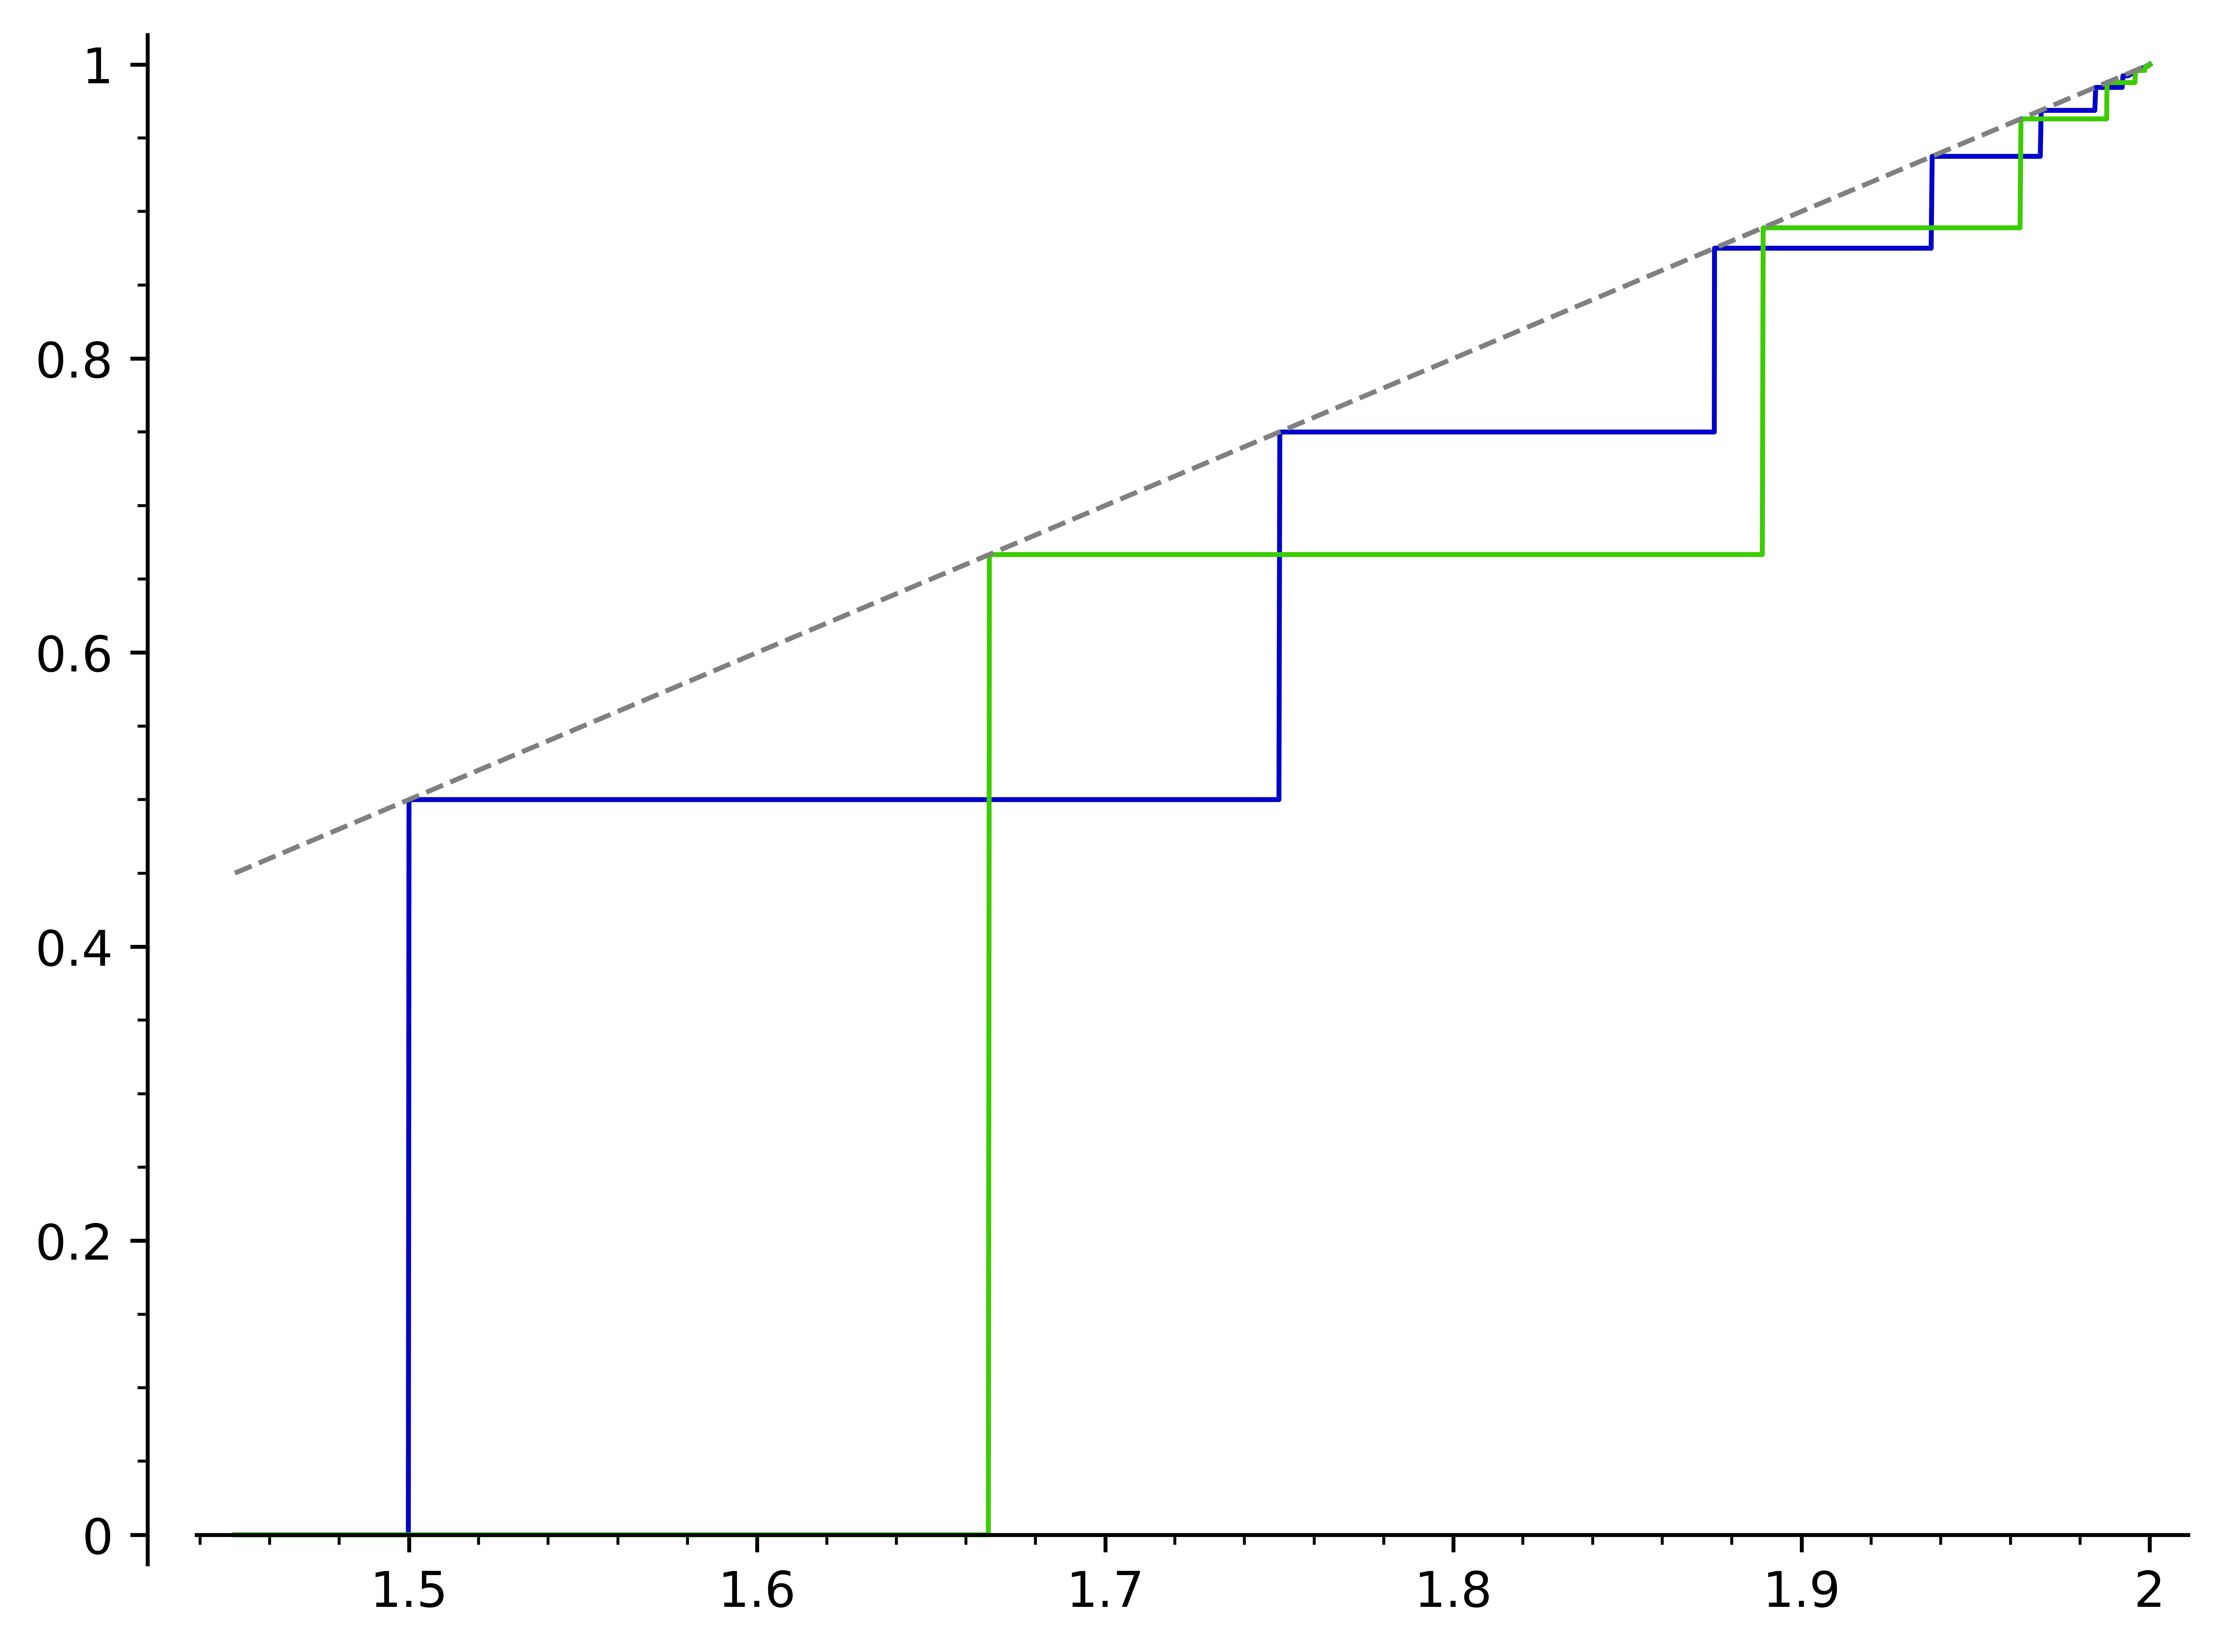
\includegraphics[width=\textwidth]{Pictures/geometric-series-distribution-2-3-half.png}
                    \caption{Geometric series construction \ref{item:geometricSeriesSufficientTailOrderConditionCounterexample}: Distribution functions $F_c$, $c=2, 3$.}
                    \label{fig:distributionsGeometricSeriesCounterexample-2-3}
                \end{subfigure}
                \begin{subfigure}[b]{0.49\textwidth}
                    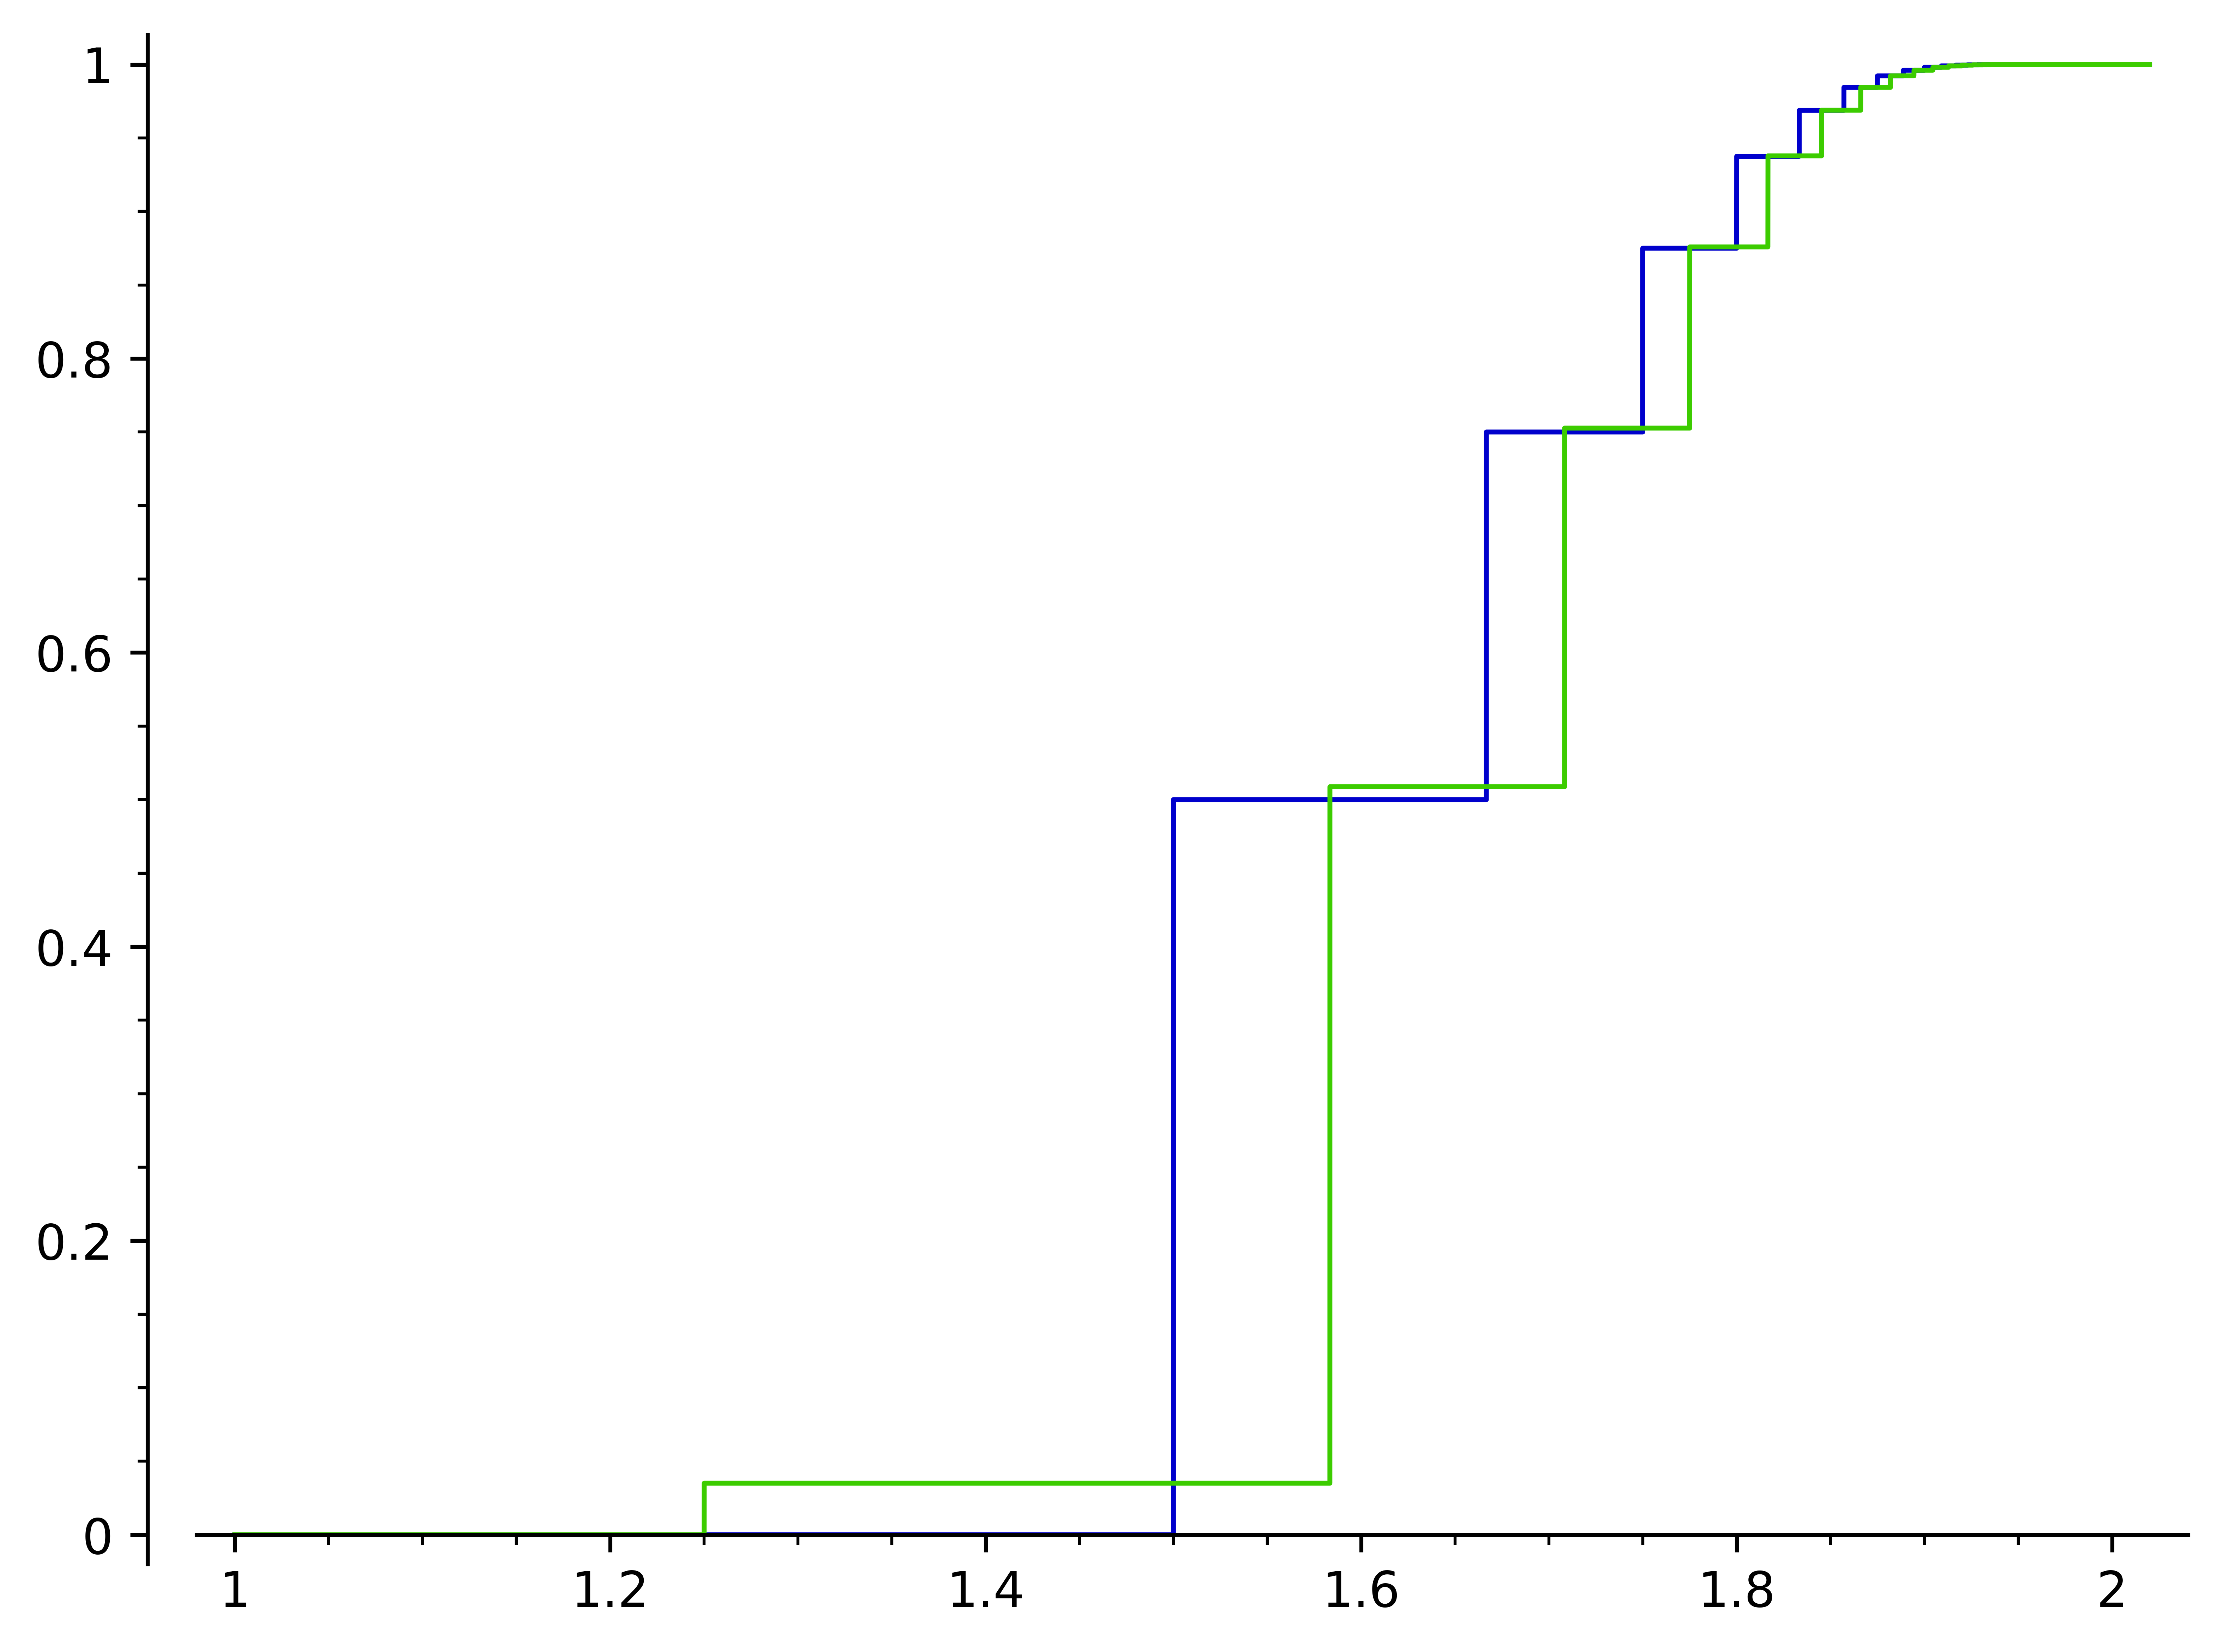
\includegraphics[width=\textwidth]{Pictures/little-shifts-distribution.png}
                    \caption{General discrete construction \ref{item:discreteSufficientTailOrderConditionCounterexample}: Distribution functions ($s_k = 1-\frac{1}{k+1}, f(s_k) = \frac{1}{2^k}$)}
                    \label{fig:littleShiftsCounterexample-distribution}
                \end{subfigure}
                
                \vspace*{0.01\textwidth}
                \begin{subfigure}[t]{0.49\textwidth}
                    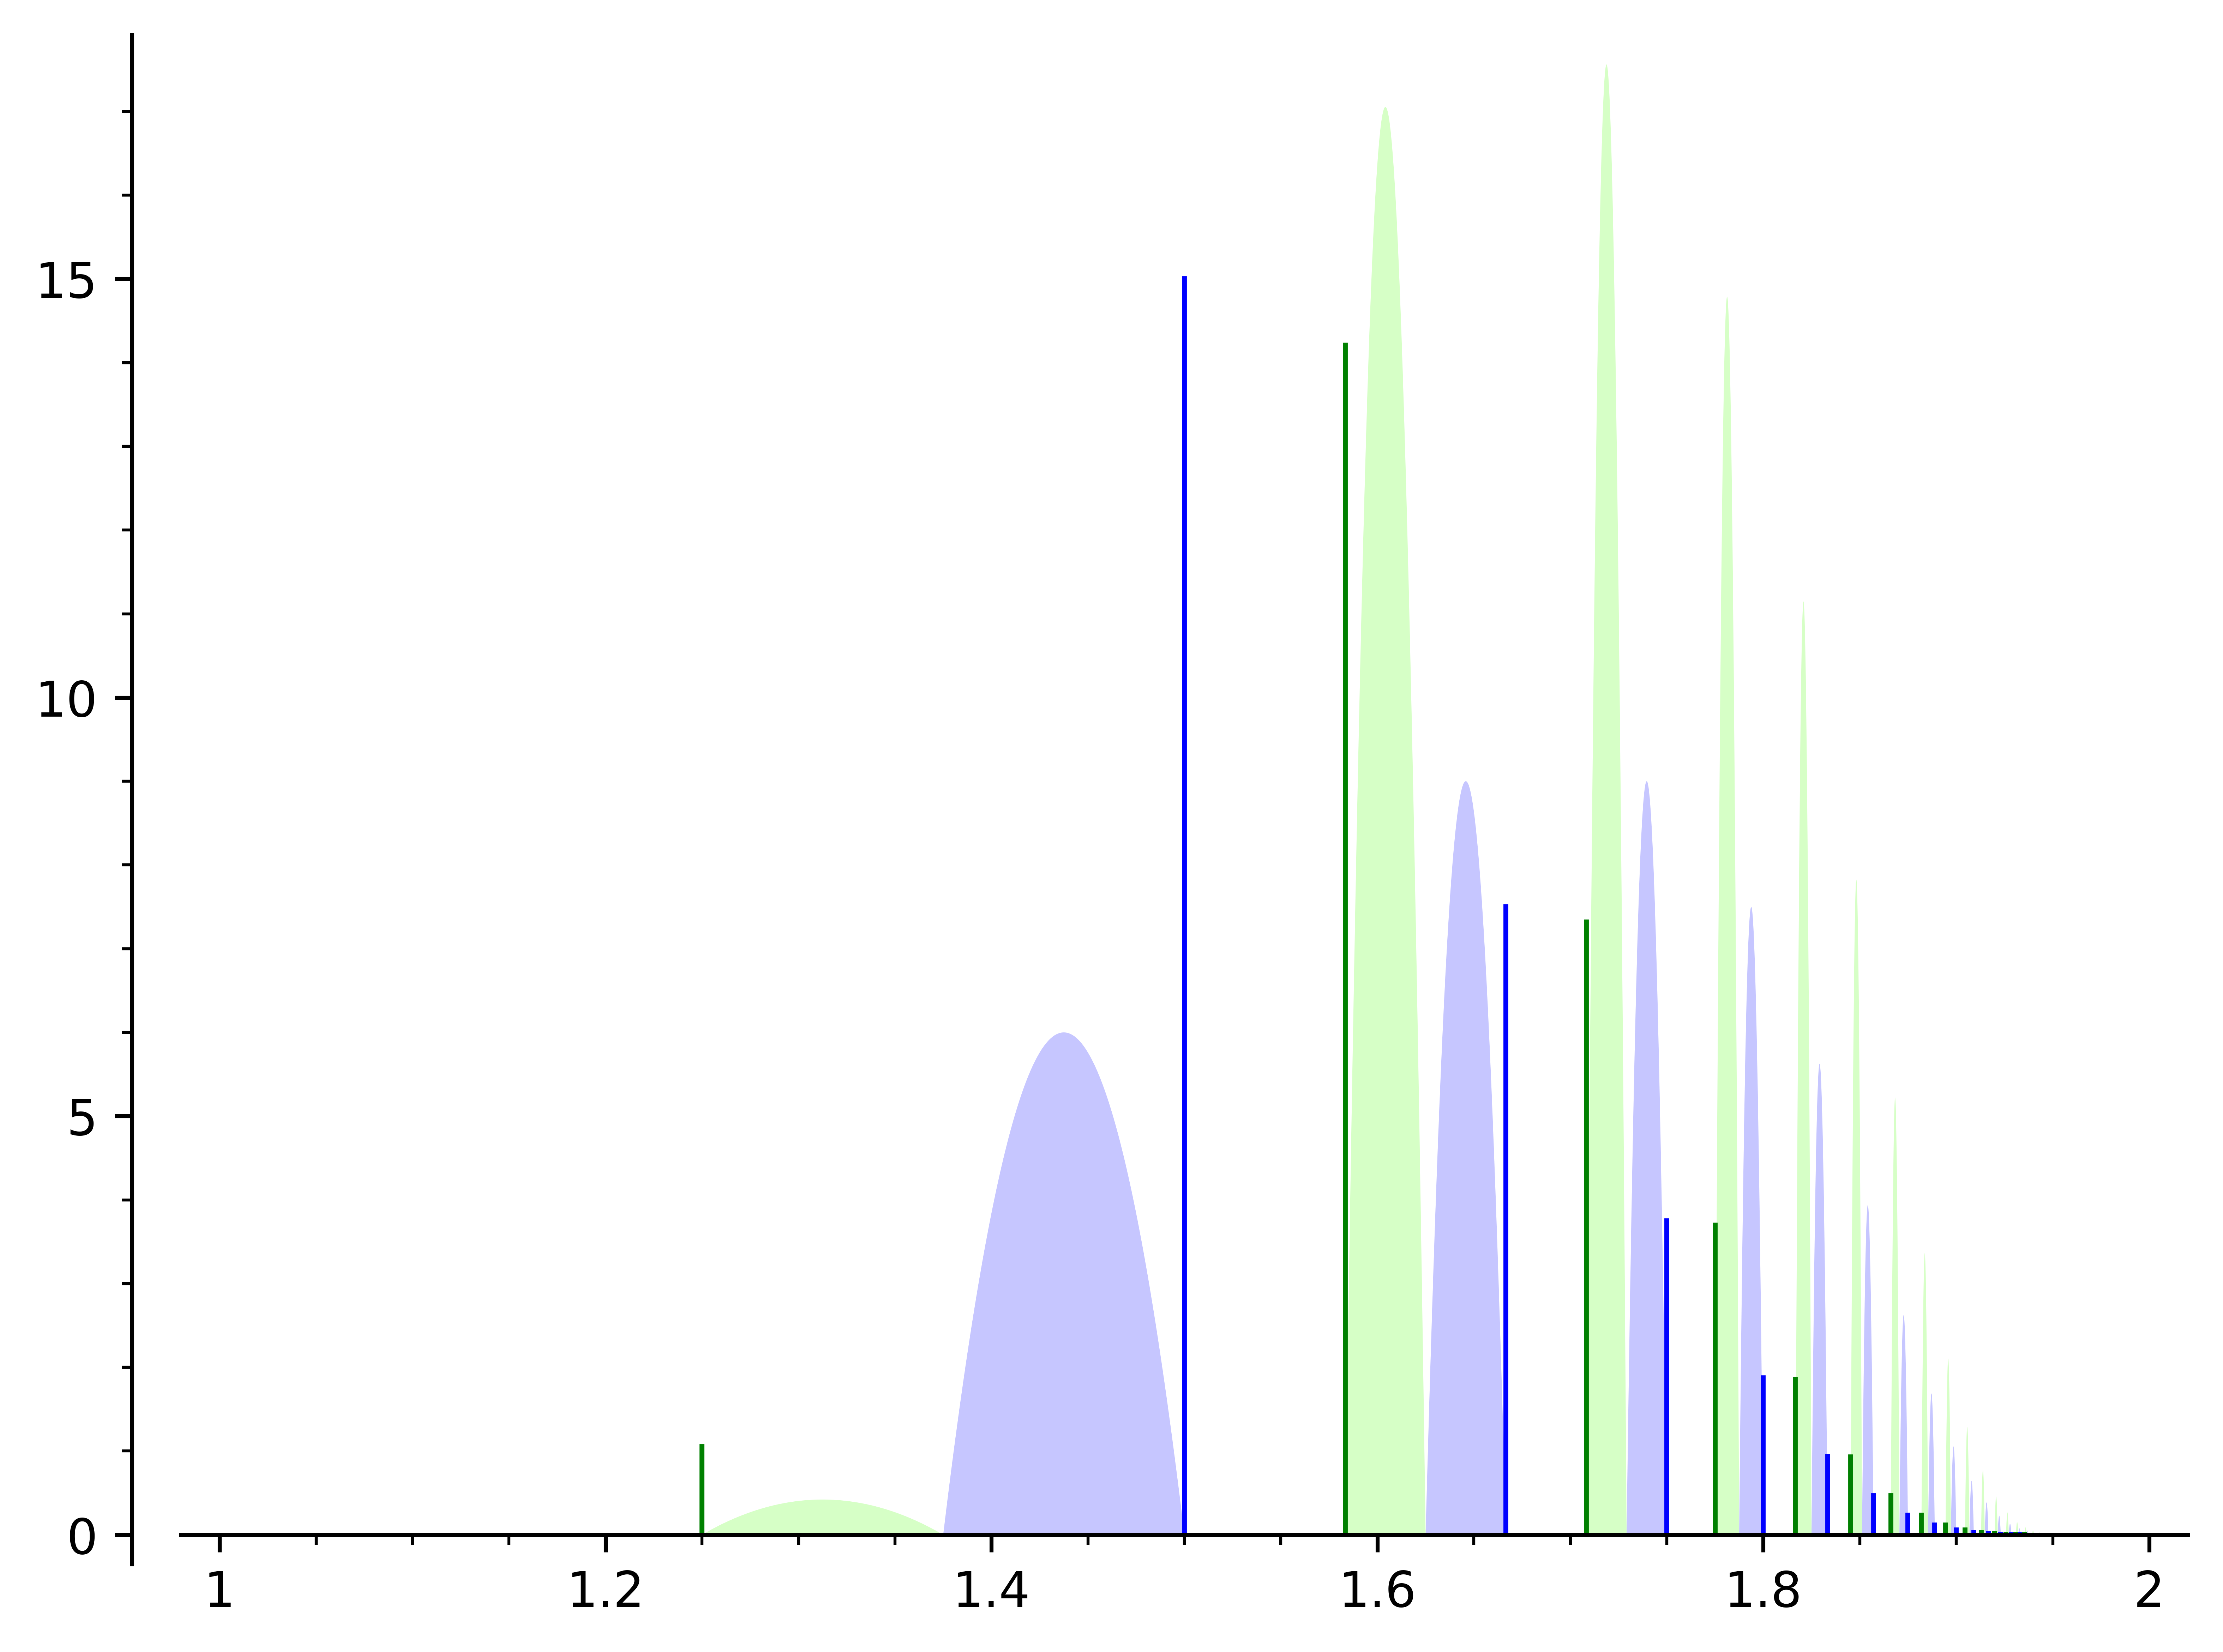
\includegraphics[width=\textwidth]{Pictures/ac-densities-masses.png}
                    \caption{Absolutely continuous construction: Densities (\ref{item:acSufficientTailOrderConditionCounterexample})/corresponding mass functions (\ref{item:discreteSufficientTailOrderConditionCounterexample}), scaled by a factor of 30}
                    \label{fig:acCounterexample-masses-densities}
                \end{subfigure}
                \begin{subfigure}[t]{0.49\textwidth}
                    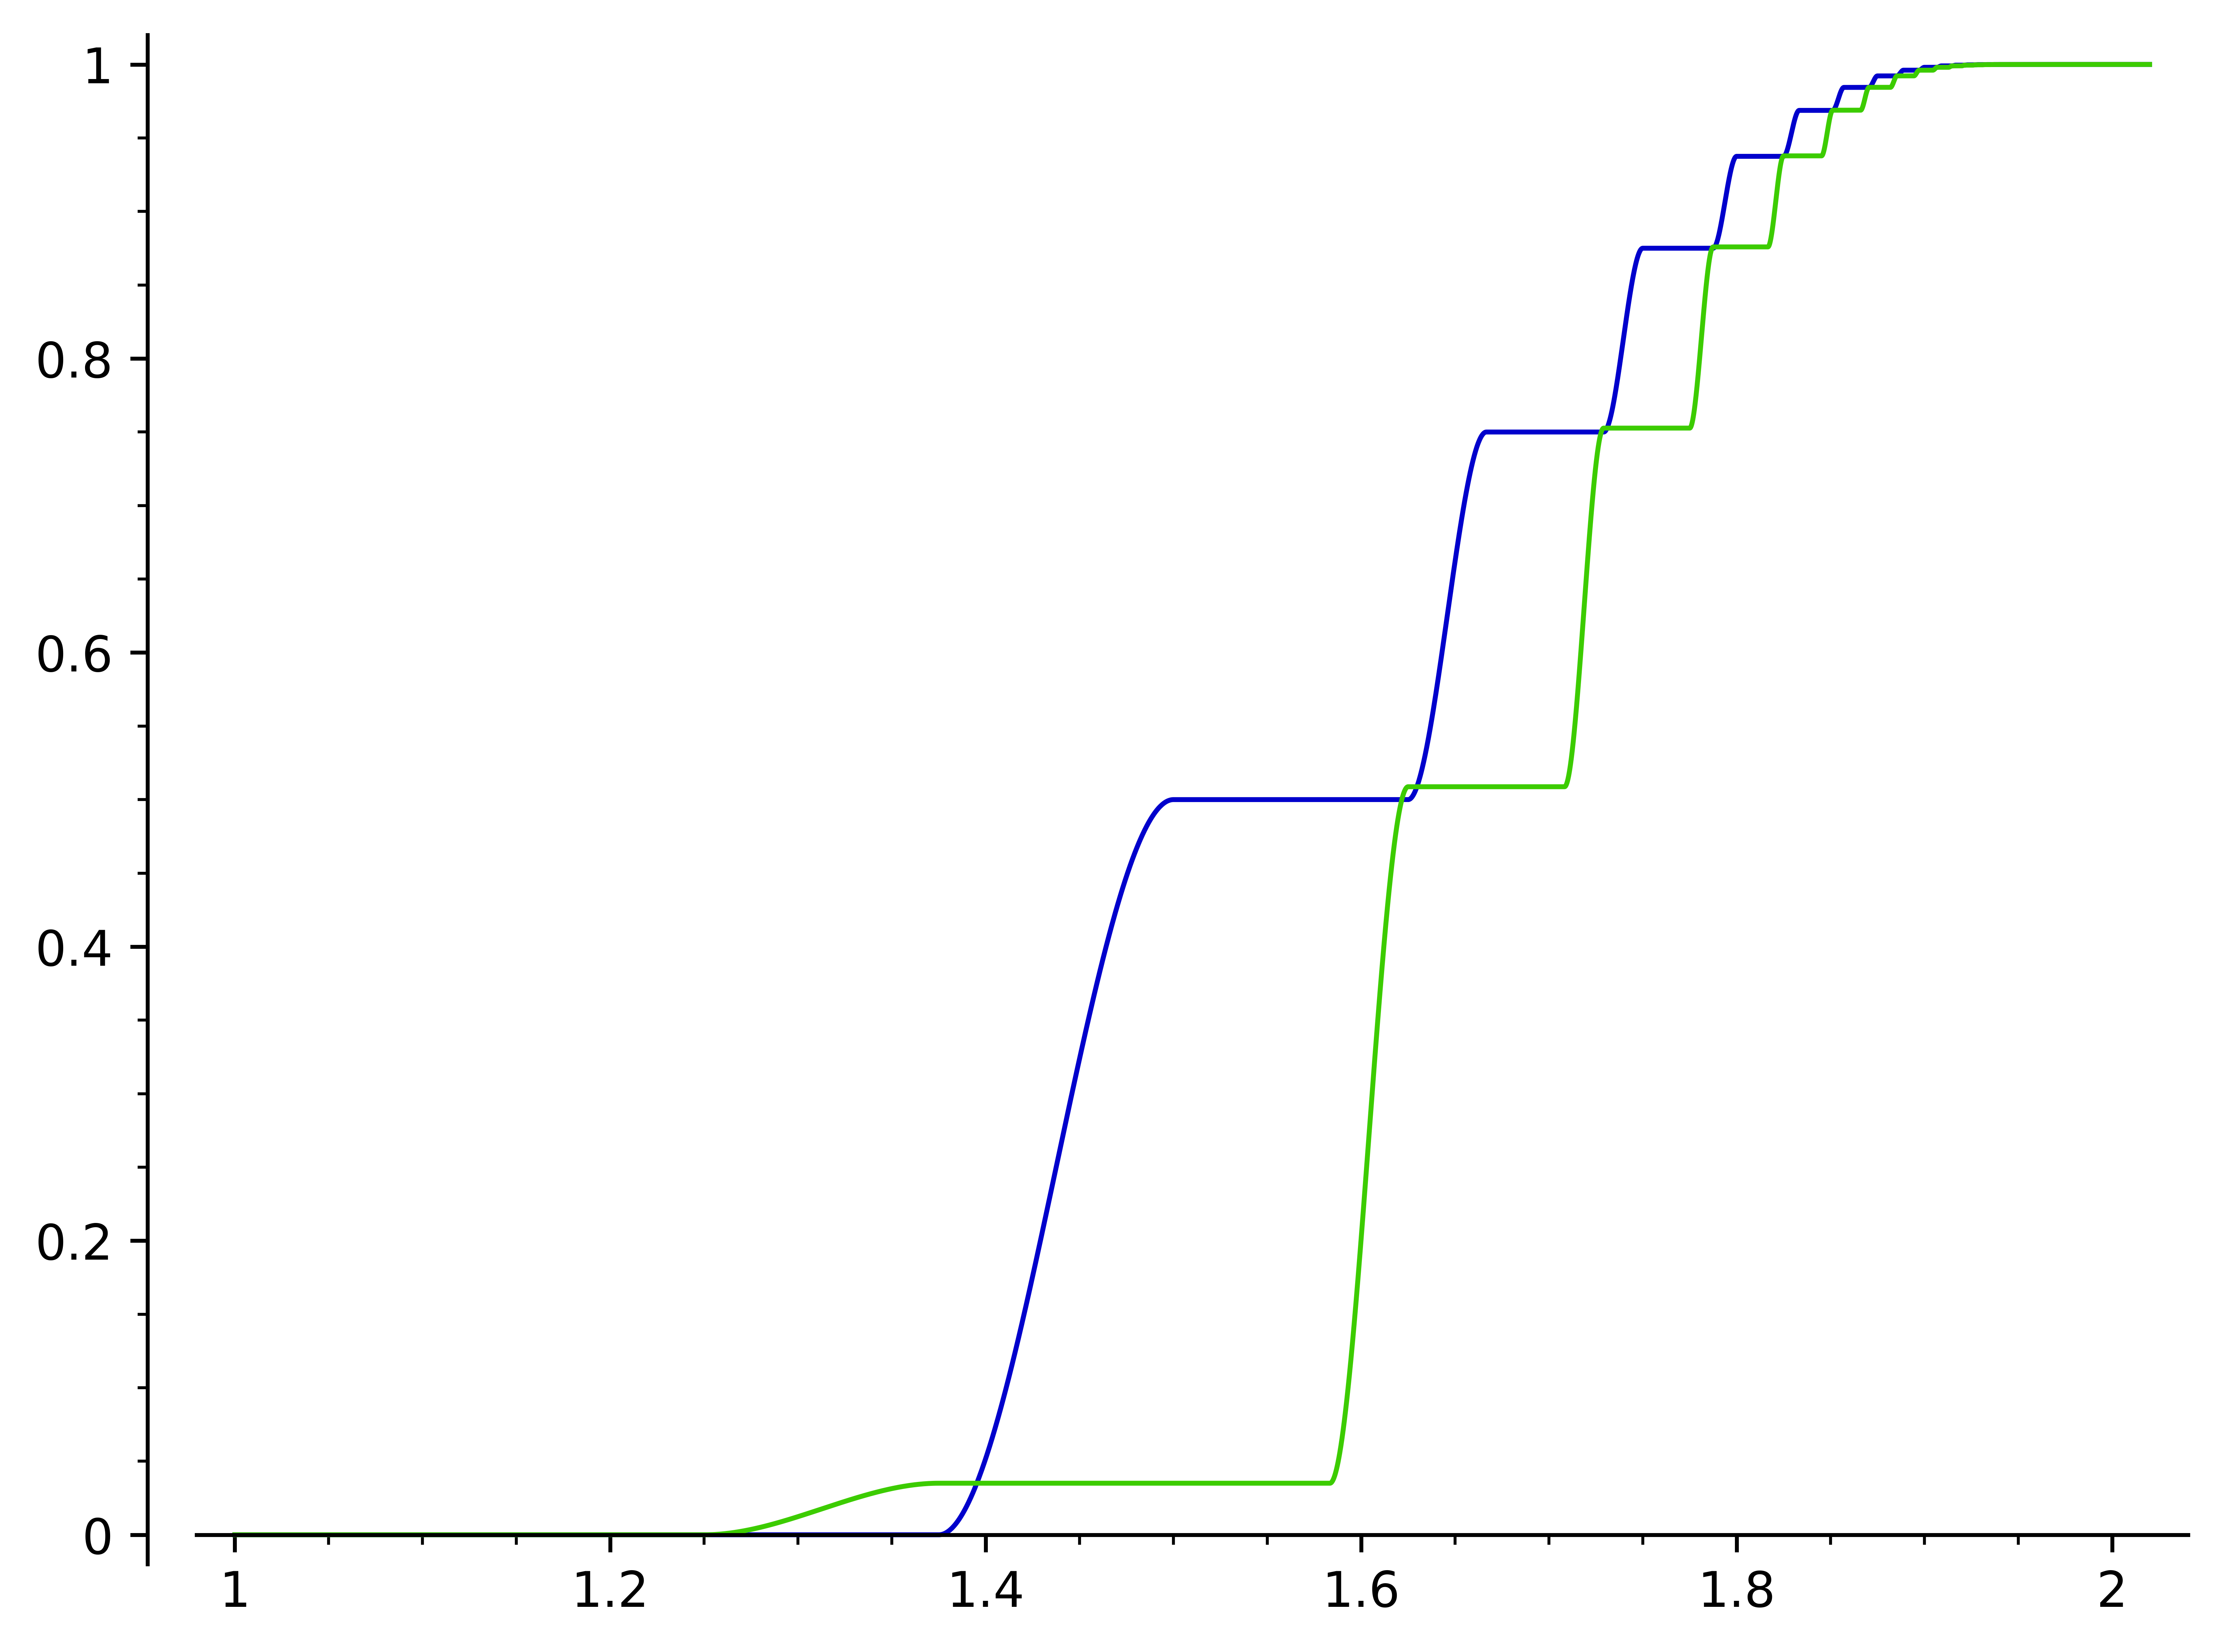
\includegraphics[width=\textwidth]{Pictures/ac-distribution.png}
                    \caption{Distribution function of absolutely continuous construction \ref{item:acSufficientTailOrderConditionCounterexample}}
                    \label{fig:acCounterexample-distribution}
                \end{subfigure}
                
                \label{fig:sufficientTailOrderConditionsCounterexamples}
                \caption{Plots for the counterexamples from Example \ref{ex:tailOrderSufficientConditionsCounterexamples}}
            \end{figure}
    
            \item 
            \label{item:discreteSufficientTailOrderConditionCounterexample}
            In another, more general approach, we start with some discrete distribution $P$ with $\supp P = \set{s_1, s_2, \dots} \subseteq [a, b)$, $1 < a < b$, the $s_i$ in increasing order, and probability mass function $f$ which is strictly decreasing on the support, i.e. $\forall i < j: f(s_i) > f(s_j)$. We construct $\tilde{P}$ with mass function $g$, where each support point is shifted a bit to the right, with its probability adjusted to be only a little smaller, giving the remaining probability mass to the point $\tilde{a} \coloneqq \frac{1+a}{2}$.
            First, set $\tilde{s}_i \coloneqq \frac{s_i+ s_{i+1}}{2}$.
            We adjust the probability of $\tilde{s}_i$ by a factor $c_i < 1$, i.e. $g(\tilde{s}_i) = c_i f(s_i)$, chosen such that $c_i \geq \frac{s_i}{\tilde{s_i}}$ (ensuring $\tilde{P}$ has greater moments than $P$), $c_i \geq 1-\frac{1}{2^i}$ (ensuring the distribution functions alternate), and $c_i \geq \frac{f(s_{i+1})}{f(s_i)}$ (ensuring that $g$ 
            also is monotonic on its support). In summary, we have:            
            \begin{gather*}
                g(\tilde{s}_i) = c_i f(s_i), \quad
                c_i \coloneqq \max\biggset{\frac{s_i}{\tilde{s_i}}, 1-\frac{1}{2^i}, \frac{f(s_{i+1})}{f(s_i)}} < 1, \quad
                g(\tilde{a}) = \sum_{i \geq 1} (1-c_i) f(s_i)
            \end{gather*}
            By the first property of $c_i$, $g(\tilde{s}_i)\tilde{s}_i \geq f(s_i)s_i ~\forall i$, so for the moments we have:
            \begin{multline*}
                m_n(\tilde{P}) - m_n(P)
                = g(\tilde{a})*\tilde{a}^n + \sum_{k \geq 1} g(\tilde{s}_i) \tilde{s}_i^n - f(s_i) s_i^n \\
                \geq g(\tilde{a}) + \sum_{k \geq 1} f(s_i) s_i^n * (\tilde{s}_i^{(n-1)} - 1)
                \geq g(\tilde{a}) > 0
%                \label{eq:momentPushingExample}
            \end{multline*}
            
            Secondly, the distribution functions alternate, see \autoref{fig:littleShiftsCounterexample-distribution}: on the one hand, 
            \begin{multline*}
                G(\tilde{s_k}) 
                = g(\tilde{a}) + \sum_{i=1}^k f(s_i)c_i 
                = g(\tilde{a}) - \bigpars{\sum_{i=1}^k (1-c_i) f(s_i)} + F(s_k) \\
                = \bigpars{\sum_{i \geq k+1} (1-c) f(s_i)} + F(s_k) > F(s_k) = F(\tilde{s_k})
            \end{multline*}
            On the other hand, 
            \begin{multline*}
                G(s_k)
                = g(\tilde{a}) + \sum_{i=1}^{k-1} f(s_i)c_i 
                = g(\tilde{a}) + \sum_{i=1}^{k-1} f(s_i) - \sum_{i=1}^{k-1} f(s_i) (1-c_i) \\
                = F(s_k) - f(s_k) + g(\tilde{a}) - \sum_{i=1}^{k-1} f(s_i) (1-c_i) 
                = F(s_k) - f(s_k) + \sum_{i \geq k} f(s_i) (1-c_i)
            \end{multline*}
            Using the second property of $c_i$ and monotonicity of $f$, we get
            $\sum_{i \geq k} f(s_i) (1-c_i) \leq \sum_{i \geq k} f(s_i) \frac{1}{2^i} < \frac{1}{2^{k-1}} f(s_k) \leq f(s_k)$,
            therefore $G(s_k) < F(s_k)$.
            So $P \lesstail \tilde{P}$, and their probability mass, as well as distribution functions are infinitely alternating, such that the sufficient condition of Theorem \ref{thm:acTailOrderSuffConditions} is not satisfied for any $x_0$.
            Furthermore, $\tilde{P}$ again satisfies the conditions we originally made on $P$: by repeating the process, we get a whole sequence of distributions which is ascending wrt. $\lesstail$, and no two distribution in it satisfy the sufficient condition of \ref{thm:acTailOrderSuffConditions} (and for any two \emph{consecutive} elements, the distribution functions are infinitely alternating as well).
            
            \item 
            \label{item:acSufficientTailOrderConditionCounterexample}
            For the absolutely continuous counterexample, we start with two discrete distributions $P_1, P_2$ where $P_2$ is obtained from $P_1$ by the process from \ref{item:discreteSufficientTailOrderConditionCounterexample}: In particular, we require $P_1 \lesstail P_2$, $\supp(P_1) = \set{s_1, s_2, \dots}$, $\supp(P_2) = \set{t_0, t_1, t_2, \dots}$ with $1 < t_0 < s_1 < t_1 < s_2 < t_2 < \dots$ ($t_0$ represents $\tilde{a}$ from above), and their distribution functions $F, G$ should alternate with $F(s_k) > G(s_k), F(t_k) < G(t_k) ~\forall k\geq 1$.
%            their mass functions $f, g$ should satisfy $f(s_i)s_i < g(t_i)t_i ~ \forall i$ (and therefore 
            
            We then shift the probability mass $P_1$ gives to each point $s_k$ to an interval to the left of $s_k$, and the probability mass $P_2$ gives to each point $t_k$ to an interval to the right of $t_k$, which preserves the order of the moments (illustrated in \autoref{fig:acCounterexample-masses-densities}). We do it in such a way that the distribution functions are again alternating, and the new density functions are continuous (\autoref{fig:acCounterexample-distribution}). We will call the new absolutely continuous distributions $\tilde{P}_1, \tilde{P}_2$, their new density functions $\tilde{f}, \tilde{g}$, and their distribution functions $\tilde{F}, \tilde{G}$.
            
            To formalize this, let $h: \R \to \R, x \mapsto (6x - 6x^2)\1_{[0, 1]}(x)$. $h$ is a simple probability density function ($\lintegral{\R}{h}{\lambda} = 1$), which is continuous since $h(0) = h(1) = 0$.
            Denote by $h_{[a, b]}: x \mapsto \frac{1}{b-a}h\bigpars{\frac{x-a}{b-a}}$ the version of $h$ scaled to the interval $[a, b]$, still integrating to 1.
%            Define $h_{a, b, s}: x \mapsto s*h(\frac{x-b}{b-a})*s$.
%            Another way to view it is that the integral of $h$ continuously interpolates between the values 0 and 1 on the interval $[0, 1]$.
            Also, let $m_{k} = \frac{t_{k-1} + s_k}{2}$.
            Using this notation, we define $\tilde{f}, \tilde{g}$ by:
            \begin{gather}
                \tilde{f} = \sum_{k \geq 1}  f(s_k) h_{[m_k, s_k]}, \quad
                \tilde{g} = \sum_{k \geq 0}  g(t_k) h_{[t_k, m_{k+1}]}
                \label{eq:acSufficientTailOrderConditionCounterexample-densitiesDefinition}
            \end{gather}
            By construction, it's clear that $\lintegral{\R}{\tilde{f}}{\lambda} = \lintegral{\R}{\tilde{g}}{\lambda} = 1$, since $(f(s_k))_{k \geq 1}, g(t_k))_{k \geq 0}$ sum to $1$. The distribution functions are alternating:
            For $k \geq 1$,
            \begin{gather*}
                \tilde{F}(s_k) 
                = \lintegral{[1, s_k]}{\tilde{f}}{\lambda} 
                = \sum_{i=1}^{k} f(s_k) 
                = F(s_k)
                > G(s_k)
                = \sum_{i=1}^{k-1} g(t_k) 
                = \tilde{G}(s_k)
                ,\\                
                \tilde{G}(m_{k+1})                
                = \lintegral{[1, m_{k+1}]}{\tilde{g}}{\lambda} 
                = \sum_{i=1}^{k} g(t_k)
                = G(t_k)
                > F(t_k)
                = \sum_{i=1}^{k} f(s_k) 
                = \tilde{F}(m_{k+1})
            \end{gather*}
            The ordering of the moments is preserved:
            \begin{multline*}
                m_n(\tilde{P_1})
                = \sum_{k \geq 1} \lintegral{[m_k, s_k]}{x^n h_{[m_k, s_k]}(x)}{\lambda(x)}
                < \sum_{k \geq 1} f(s_k)*s_k^n \\
                = m_n(P_1)
                < m_n(P_2) \\
                = \sum_{k \geq 0} g(t_k)*t_k^n
                < \sum_{k \geq 0} \lintegral{[t_k, m_{k+1}]}{x^n h_{[t_k, m_{k+1}]}(x)}{\lambda(x)}
                = m_n(\tilde{P_2})
            \end{multline*}
            If the series in \eqref{eq:acSufficientTailOrderConditionCounterexample-densitiesDefinition} converges uniformly, continuity is preserved.
            For this we additionally need to have $\norm{f(s_k) h_{[m_k, s_k]}}_\infty = \frac{f(s_k)}{s_k - m_k} \toinfty{k} 0$, and similarly for $g$, which is the case if the probability masses $f(s_k)$ approach zero asymptotically faster than the consecutive differences of the $s_k$. For example, we can set $s_k = 2-\frac{1}{k+1}, f(s_k) = \frac{1}{2^k}$, and use $g, (t_k)_k$ constructed from it as in \ref{item:discreteSufficientTailOrderConditionCounterexample}.
            % TODO properly reference “uniform convergence preserves continuity”
        \end{enumerate}
    \end{ex}
    
    \subsection{Totality of Restricted Versions of the Tail Order}
    When we introduced the tail order, we already discussed its anti-symmetry and totality properties: In short, $\leqtail$ in general is neither total nor anti-symmetric; For anti-symmetry, good counterexamples of distributions with equal moment sequences exist, however anti-symmetry \emph{does} hold on the reasonably large subset of distributions with bounded support.
    For totality, the situation is less clear: the only counterexamples we saw so far were trivially not $\leqtail$-comparable because they did not even have moments of all orders.
    A natural question thus is if there is some useful subset of $\DP$ where $\leqtail$ is total. Most generally, is $\leqtail$ total on $L$, i.e. are distributions comparable as soon as  they have moments of all orders? This first question is easy to answer: $\leqtail$ is not total on the whole of $L$, because distributions can take negative values that can make the moment sequences alternating. 
    % TODO make this “alternating moment sequences” example even shorter [using Dirac measure notations]. Maybe  even move it further up, to the definition of tail order, discussing that \leqtail is not useful on negative values in the support
    As the simplest example, consider the point-mass distributions on $-1$ and $0$: The moment sequence of the former is given by $(-1)^n$, alternating around the sequence of the latter which is constantly $0$, making the distributions not $\leqtail$-comparable.
    However, a more realistic question is: is there a smaller subset of $\DP$ where $\leqtail$ is total, which is easy to characterize and big enough to contain many useful distributions?
    
    In \cite{bib:rassGameRiskManagI,bib:rassTotalOrderingOnLossDistributions}, the discussion focuses on the particular subset of distributions that have \emph{bounded support which is a subset of $[1, \infty)$} and are either \emph{discrete with finite support}, or \emph{absolutely continuous with a continuous density function}.
    In \cite[Lemma 2]{bib:rassTotalOrderingOnLossDistributions} and \cite[Lemma 2.4]{bib:rassGameRiskManagI}, the claim is that such distributions are always $\leqtail$-comparable.
    A proof is given for the absolutely continuous case; however, it contains an error, as it applies an argument similar to Theorem \ref{thm:acTailOrderSuffConditions} and implicitly assumes that of two density functions, one dominates the other from some point on
    \footnote{Meanwhile, the error was fixed in \cite{bib:rassGameRiskManagI}, and a new version was uploaded to arxiv stating all requirements.}.
    As shown in Example \ref{ex:tailOrderSufficientConditionsCounterexamples}, pairs of distributions exist where this is not the case, and which also are in $\Fgeq$, bounded, and have continuous density functions.
    
    \subsubsection{The Moment Problem and its Variants}
    Since our question crucially depends on properties of moment sequences, it will be helpful to know about the properties of moment sequences.
    The question to find out whether a given sequence $(m_n)_n$ is a moment sequence for some Borel measure $\mu$ on $\R$ is known as the \emph{moment problem}, and there are several variants studied in the literature:
%    to characterize moment sequences is known as the \emph{moment problem}, and there are several variants:
    The \emph{Hamburger moment problem} concerns measures supported on a subset of $\R$, the \emph{Stieltjes moment problem} is about measures supported on a subset of $[0, \infty)$,
    and the \emph{Hausdorff moment problem} deals with measures supported on a subset of $[0, 1]$. For all three versions, conditions are known that are both sufficient and necessary for $(m_n)_n$ to be a moment sequence of the respective kind.
    There is extensive literature on the subject, for example \cite{bib:shohatTheProblemOfMoments}, \cite{bib:akhiezerClassicalMomentProblem}, or the more modern \cite{bib:schmuedgenTheMomentProblem}.
    The Hamburger moment problem is too general for our case, since negative values in the support can lead to alternating moment sequences, making the tail order non-total.
    % TODO and negative values in the support make it useless, too.
%    We will introduce the characterizations by Stieltjes and Hausdorff, which are more interesting for us.
%    
%    \begin{defn}
%        % TODO check if the term “Hankel matrix” is appropriate. Isn't that an infinite matrix?
%        Let $n \geq 1$, $a_0, a_1, \dots, a_{2n} \in \R$. Define the \emph{Hankel matrix} $H(a_0,\dots,a_{2n})$ as
%        \begin{gather*}
%            H(a_0,\dots,a_{2n}) \coloneqq
%            \begin{pmatrix}
%            	a_0    & a_1     & a_2    & \dots    & a_n      \\
%            	a_1    & a_2     & \ddots &          & a_{n+1}  \\
%            	a_2    & \ddots  & \ddots & \ddots   & \vdots   \\
%            	\vdots &         & \ddots & \ddots   & a_{2n-1} \\
%            	a_n    & a_{n+1} & \dots  & a_{2n-1} & a_{2n}
%            \end{pmatrix}
%            \in \R^{(n+1)\times(n+1)}
%        \end{gather*}
%    \end{defn}
%    
%    \begin{thm}[Stieltjes Moment Characterization]
%        A sequence $(m_n)_{n \geq 0}$ of real numbers is the moment sequence of some measure $\mu$ on $[0, \infty)$ if and only if one of the following conditions hold:
%%        \begin{enumerate}
%%            \item
%%            \begin{gather*}
%%                
%%            \end{gather*}
%%        \end{enumerate}
%        \begin{gather}
%            \forall n: \det(H(m_0, \dots, m_{2n})) > 0,~ \det(H(m_1, \dots, m_{2n+1})) > 0 \\
%            \begin{split}
%                \forall n \geq m: \det(H(m_0, \dots, m_{2n})) > 0,~ \det(H(m_1, \dots, m_{2n+1})) > 0 \\
%                \text{ and } \forall n > m: \det(H(m_0, \dots, m_{2n})) = \det(H(m_1, \dots, m_{2n+1})) = 0
%            \end{split}
%        \end{gather}
%        In the first case, the measure $\mu$ has infinite support, in the second case, it has finite support of size $m$.
%    \end{thm}  

    \subsubsection{Non-Totality in the Stieltjes Case}
    However, we can make use of a result relating Stieltjes and Hamburger moment sequences:
    A moment sequence is called \emph{Hamburger-}/\emph{Stieltjes-}/\emph{Hausdorff-determinate} if there is a \emph{unique} measure of the respective type generating the sequence. The result we'll use is that Stieltjes-determinateness in general does not imply Hamburger-determinateness:
    
    \begin{thm}[See \cite{bib:linMomentProblemRecentDevelopments}, in turn citing {\cite[p.240]{bib:akhiezerClassicalMomentProblem}} and \cite{bib:chiharaIndeterminateHamburgerMomentProblems}]
        % TODO cite Akhiezer/Dong Lin/Chihara
        There exists a moment sequence $(m_n)_{n \geq 0}$ that is Stieltjes-determinate, but not Hamburger-determinate.
    \end{thm}

    \begin{cor}
        There exist probability measures $P_1, P_2$ with equal moment sequences, where $\supp (P_1) \subseteq [0, \infty)$ and $\supp (P_2) \subsetneq [0, \infty)$.
        \label{cor:equalMomentSequencesStieltjesHamburger}
    \end{cor}
    \begin{proof}
        Let $(m_n)_{n \geq 0}$ be a moment sequence which is Stieltjes-determinate, but not Hamburger-determinate.
        Let $\mu_1$ be the unique measure with that moment sequence and support in $[0, \infty)$.
        Let $\mu_2 \neq \mu_1$ be a different measure with that moment sequence, which exists since the sequence is not Hamburger-determinate. 
        Since $\mu_1$ is unique in the Stieltjes sense, the support of $\mu_2$ must overlap with $(-\infty, 0)$.
        If $m_0 \neq 1$, the measures constructed are not probability measures: 
        We set $P_1 = \frac{1}{m_0}\mu_1, P_2 = \frac{1}{m_0}\mu_2$, which are probability measures which both have the moment sequence $(\frac{m_n}{m_0})_{n \geq 0}$.
    \end{proof}
    
    This result allows us to show that two Stieltjes moment sequences can infinitely alternate: 
    \begin{ex}
%        We construct a pair of probability measures supported on a subset of $[0, \infty)$, which have infinitely alternating moment sequences:
        Let $P_1, P_2$ be the measures from Corollary \ref{cor:equalMomentSequencesStieltjesHamburger}, with moment sequence $(m_n)_{n \geq 0}$.
        Define a measure $\tilde{P}_2: A \mapsto P_2(A \cap [0, \infty)) + \1_A(0) P_2((\infty, 0))$, which shifts the whole probability mass $P_2$ puts on the negative half-axis to the point $0$, and has support in $[0, \infty)$.
        Then its moment sequence $(\tilde{m}_n)_{n \geq 0}$ is given by $\tilde{m}_0 = 1$, and for $n > 0$:
        \begin{gather*}
            \tilde{m}_n 
            = \lintegral{[0, \infty)}{x^n}{\tilde{P}_2}
            = \lintegral{[0, \infty)}{x^n}{P_2}
            = \lintegral{\R}{x^n}{P_2} - \lintegral{(-\infty, 0)}{x^n}{P_2}
            = m_n - \undersetbrace{\lintegral{(-\infty, 0)}{x^n}{P_2}}{\text{alternating}}
        \end{gather*}
        By construction of $P_2$, the term $\lintegral{(-\infty, 0)}{x^n}{P_2}$ is strictly positive for $n$ even, and strictly negative for $n$ odd.
        Therefore $(\tilde{m}_n)_{n \geq 0}$ alternates infinitely around $(m_n)_{n \geq 0}$,
        and both sequences are moment sequences of probability measures supported on a subset of $[0, \infty)$.
    \end{ex}

    This shows that the space of probability measures supported on a subset of $[0, \infty)$ that have moments of all orders is still too large for $\leqtail$ to be total.
    \todo{Give a counterexample explicitly.}
    
    \subsubsection{Distributions with Non-Negative Bounded Support}
    Next we look at distributions with support in a bounded interval $[a, b]$, $0 \leq a < b$.
    This is related to the Hausdorff moment problem where the bounded interval is $[0, 1]$.
    A sufficient and necessary condition for a sequence to be a Hausdorff moment sequence is based on repeatedly taking differences of successive terms.
    \begin{defn}
        The \emph{difference operator} $\Delta: \R^{\N_0} \to \R^{\N_0}$ maps a sequence of real numbers to the sequence of its successive differences:
        \[
            \Delta((s_n)_{n \in \N_0}) \coloneqq (s_{n+1} - s_n)_{n \in \N_0}, ~ \text{ also written as }\,
            (\Delta s)_n \coloneqq s_{n+1} - s_n
        \]
    \end{defn}

    \begin{thm}[\cite{bib:hausdorffMomentprobleme}]
        A sequence $m = (m_n)_{n \in \N_0}$ is a Hausdorff moment sequence, i.e. is the moment sequence of a measure $\mu$ on with support in $[0, 1]$,
        if and only if
        \begin{gather}
            \forall n, k \in \N: (-1)^k (\Delta^k m)_n \geq 0
            \label{eq:completelyMonotonicSequence}
        \end{gather}
        A sequence satisfying \eqref{eq:completelyMonotonicSequence} is also called \emph{completely monotonic}.
        \label{thm:hausdorffMomentSequenceCharacterization}
    \end{thm}
    \begin{proof}[Proof (necessity)]
        We only show here that condition \eqref{eq:completelyMonotonicSequence} is necessary, which is the easier part of the proof.
        Let $\mu$ be the measure with support in $[0, 1]$ which has $m$ as its moment sequence.
        We first proof by induction over $k$ that $(\Delta^k m)_n = \lintegral{[0, 1]}{x^n (x-1)^k}{\mu(x)}$:
        \begin{gather*}
            (\Delta m)_n 
            = m_{n+1} - m_{n} 
            = \lintegral{[0, 1]}{x^{n+1}}{\mu(x)} - \lintegral{[0, 1]}{x^n}{\mu(x)} 
            = \lintegral{[0, 1]}{x^n(x-1)}{\mu(x)}, \\
            (\Delta^{k+1} m)_n
%            = (\Delta^k m)_{n+1} - (\Delta^k m)_n \\
            = \lintegral{[0, 1]}{x^{n+1} (x-1)^k}{\mu(x)} - \lintegral{[0, 1]}{x^n (x-1)^k}{\mu(x)}
            = \lintegral{[0, 1]}{x^{n}(x-1)^{k+1}}{\mu(x)}
        \end{gather*}
        From this we directly get that $(-1)^k (\Delta^k m)_n = \lintegral{[0, 1]}{x^n (1-x)^k}{\mu(x)}$.
        Since we integrate over $[0, 1]$, the integrand is non-negative on the domain of integration.
        Therefore, $(-1)^k (\Delta^k m)_n \geq 0$.
    \end{proof}

    However, our focus is not so much on distributions with support in $[0, 1]$, but rather with support in $[1, b]$ for some $b > 1$.
    Moment sequences behave somewhat differently in that case: While they are monotonically decreasing in the former case, they are monotonically increasing in the latter, even growing without bound if there is some mass to the right of $1$.
    Yet we can obtain a necessary criterion looking similar to \eqref{eq:completelyMonotonicSequence} for a sequence to be the moment sequence of such a distribution:
    \begin{cor}
        \label{cor:hausdorff-1-b-necessaryCondition}
        For any moment sequence $m$ of a measure $\mu$ supported on a subset of $[1, b]$, all successive differences are non-negative:
        \begin{gather}
            \forall n, k \in \N: (\Delta^k m)_n \geq 0
        \end{gather}
    \end{cor}
    \begin{proof}
        Just as in the last proof, we have that $(\Delta^k m)_n = \lintegral{[1, b]}{x^n (x-1)^k}{\mu(x)}$.
        Since in this case, $x-1 > 0 \,\forall x \in [1, b]$, the integrand is non-negative, and $(\Delta^k m)_n \geq 0$.
    \end{proof}

    Another similar necessary condition can be stated for moment sequences of distributions on $[0, b]$, using a somewhat modified difference operator:
    \newcommand{\DeltaB}[1]{\Delta\hspace{-.225cm}{\mathrel{\raisebox{0.045cm}{\scalebox{.9}{$\scriptscriptstyle#1$}}}\hspace{.22cm}}}
    \begin{lemma}
        \label{lemma:hausdorff-0-b-necessaryCondition}
        Let $\DeltaB{b}: \R^{\N_0} \to \R^{\N_0}$, $(\DeltaB{b} m)_n \coloneqq m_{n+1} - b * m_n$.
        Then for any moment sequence $m$ of a measure $\mu$ supported on a subset of $[0, b]$:
        \begin{gather}            
            \forall n, k \in \N: (-1)^k (\DeltaB{b}^k m)_n \geq 0
        \end{gather}
    \end{lemma}
    \begin{proof}
        Analogously to the proof of \ref{thm:hausdorffMomentSequenceCharacterization},
        we can prove by induction that $(\DeltaB{b}^k m)_n = \lintegral{[0, b]}{x^n (x-b)^k}{\mu(x)}$.
        Since again, in $(-1)^k (\DeltaB{b}^k m)_n = \lintegral{[0, b]}{x^n (b - x)^k}{\mu(x)}$, the integrand is non-negative, we can conclude $(-1)^k (\DeltaB{b}^k m)_n \geq 0$.
    \end{proof}

    % TODO basically, we woould need a sufficient condition to construct a counterexample; if we can proof that no alternating counterexample exists, a necessary condition will be enough.
    While \ref{cor:hausdorff-1-b-necessaryCondition} and \ref{lemma:hausdorff-0-b-necessaryCondition} give necessary conditions, it would be very useful to have a condition that is also sufficient. However, using \ref{lemma:hausdorff-0-b-necessaryCondition} we can show that \ref{cor:hausdorff-1-b-necessaryCondition} can not be a sufficient condition, as the next example shows.
    
    \begin{ex}
        We construct a sequence that satisfies the condition of \ref{cor:hausdorff-1-b-necessaryCondition} and is infinitely alternating around a moment sequence:
        Let sequences $s, q$ be given by $s_n = 4^n$, $q_n = (-1)^n\frac{1}{2^n}$, $n \in \N_0$. $s$ is clearly a moment sequence; we show that $(s_n + q_n)_{n \in \N_0}$ satisfies the conditions of \ref{cor:hausdorff-1-b-necessaryCondition}:
        By induction, one can show that $(\Delta^k s)_n = 3^k 2^n$ and $(\Delta^k q)_n = 3^k\frac{(-1)^{n+k}}{2^{n+k}}$.
        Since the $\Delta$-operator is linear, we have $(\Delta^k (s+q))_n = 3^k\bigpars{2^n + \frac{(-1)^{n+k}}{2^{n+k}}} \geq 0$ for all $n, k$.
        So $s+q$ is infinitely alternating around the moment sequence $s$ and satisfies \ref{cor:hausdorff-1-b-necessaryCondition}, which would make it a candidate for a counterexample to the tail order being total for non-negative bounded distributions. 
        
        However, $s+q$ does not satisfy \ref{lemma:hausdorff-0-b-necessaryCondition} for any reasonable choice of $b$:
        If $s+q$ was the moment sequence of some measure $\mu$ with support in $[0, b]$, then $\forall n \geq 0: s_n + q_n < b^n$.
        We can take the generous bound $s_n + q_n \leq 5^n$ which is satisfied, since $s_n \leq 4^n, q_n < 1$ - so the support of $\mu$ would definitely be a subset of $[0, 5]$.
        However, calculations show that $(\DeltaB{5}^2 (s+q))_1 = -\frac{89}{8} < 0$, so by \ref{lemma:hausdorff-0-b-necessaryCondition}, $(s+q)$ is not a moment sequence of such a measure.
    \end{ex}

    \subsubsection{Possible Further Progress}

    As far as this thesis is concerned, the question whether two moment sequences of distributions on either an interval $[0, b]$ or an interval $[1, b]$ can be infinitely alternating could not be solved yet. It therefore remains open for the moment if $\leqtail$ is a total order on such distributions.
    However, the condition of complete monotonicity \eqref{eq:completelyMonotonicSequence} seems quite strict, and during experimentation I could not even find a pair of completely monotonic sequences alternating more than twice; some possible further progress could be to prove that two Hausdorff moment sequences (i.e. for the $[0, 1]$-case) can not infinitely alternate. Possibly, such a result could be easily generalized to the $[0, b]$-case using the condition of \ref{lemma:hausdorff-0-b-necessaryCondition}; however another issue is how to generalize it to the $[1, b]$-case.
    % TODO find references that seem to suggest that Hausdorff works for [a, b] (e.g. the one book review, but more?)
    
    While the necessary condition of \ref{lemma:hausdorff-0-b-necessaryCondition} might be enough to transfer a positive result from $[0, 1]$ to $[0, b]$, it does not suffice if a counterexample is found: Even if we found two alternating sequences satisfying the conditions of \ref{lemma:hausdorff-0-b-necessaryCondition}, this would still not ensure that corresponding Borel measures exist, since the only proved the condition to be necessary, not sufficient.
    Yet another issue is that we are especially interested in distributions that 
%    either have finite support, or 
    are absolutely continuous (or with finite support, but there no counterexamples exist by \ref{thm:discreteTailOrderSuffConditions}); so even if we found a counterexample and proved that the two sequences belonged to measures on $[0, b]$, this would still not ensure the measures are absolutely continuous.
    
    An interesting note is that in some references it is suggested that Hausdorff's characterization can easily be generalized to any interval $[a, b]$ (for example, the review \cite{bib:bultheelBookReviewMomentProblem} on Schmüdgen's book \cite{bib:schmuedgenTheMomentProblem}).
    However, I could not yet find a formalization of this as a necessary and sufficient criterion. If something in this direction could be found, this would definitely be a helpful step, either for transferring a proof from $[0, 1]$ to $[1, b]$, or for proving counterexample sequences to have corresponding measures.
     
    
    \section{Equilibria in Tail-Ordered Games}
    We will now look at equilibria of distribution-valued games with respect to the stochastic tail order.
    An important result of this section is that, unlike their real-valued counterparts, these games fail to have mixed-strategy equilibria in general.
    
    We first
    % TODO do we really *first* restrict ourselves to LEX-Games, or permanently?
    restrict our attention to games with finitely supported distributions as payoffs.
    As shown in Corollary \ref{cor:discreteFiniteTailOrder-RLexEquivalence}, for such distributions the tail order can be reduced to lexicographical comparison.
    To make our discussion notationally easier, we will represent games with finite common support of the payoff distributions as real-valued vectors of probabilities, ordered by the reflect lexicographical order.
    \begin{defn}
        A \emph{vector-valued game} of dimension $m \in \N$ is a game $G_{\leqRlex}$ with preordered payoff space $\R^m$.
        If it it equipped with the preorder $\leqRlex$, we call it a \emph{reflected-lexicographically ordered} (also \emph{ref-lex-ordered}) game.
    \end{defn}

    \begin{lemma}
        Let $G$ be a distribution valued game where $\supp(G) \coloneqq \bigcup\limits_{s \in S, 1 \leq k \leq n} \supp(u_k(s))$ is finite, 
        in particular $\supp(G) = \set{x_1, \dots, x_m}$, $x_1 < \dots < x_n$. Let $u_k(s)$ have probability mass function $f_{k, s}$.
        Define the ref-lex-ordered game $H$ with payoffs
        $v_k(s) \coloneqq (f_{k, s}(x_1), \dots, f_{k, s}(x_m))$.
        Then $G_{\leqtail}$ and $H_{\leqRlex}$ are isomorphic.
    \end{lemma}
    \begin{proof}
        The bijective function $\phi: \DP \to \R^m$ is already clear by definition of $v_k$.
        By Corollary \ref{cor:discreteFiniteTailOrder-RLexEquivalence}, mapping distributions ordered by $\leqtail$ to real-valued vectors ordered by $\leqRlex$ preserves the ordering.
    \end{proof}

    \subsection{Existence Conditions for Mixed-Strategy Equilibria in Lexicographically-Ordered Games}
    % TODO better game table design
    \begin{ex}
        \label{ex:reflectedLexicographicallyOrderedGame}
%        Consider the vector-valued two-player zero-sum game $G$ represented by
        An example of a ref-lex game could look like:
        \begin{gather}
            \centering
            \begin{tabular}{c|c|c|}
            	      &        $b_1$        &        $b_2$        \\ \hline
            	$a_1$ & (0.1,\; 0.8,\; 0.1) & (0.1,\; 0.7,\; 0.2) \\ \hline
            	$a_2$ & (0.6,\; 0.1,\; 0.3) & (0.8,\; 0.1,\; 0.1) \\ \hline
            \end{tabular}
        \end{gather}
        The game is a two-player matrix game (i.e. zero-sum), so we only specify payoffs for the first player.
        An equivalent tail-ordered distribution-valued game can be constructed from it for any specified support set of size 3;
        Which specific support is chosen however does not matter for the tail order.
%        $G$ has no mixed-strategy equilibrium with respect to $\leqtail$.
    \end{ex}

    \newcommand{\Gproj}[1]{G_{#1}}
    \newcommand{\Gprojsub}[1]{\bar{G}_{#1}}
    
    The game given in the last example has no Nash equilibria with respect to $\leqRlex$.
    To see this we will first take a closer look at the highest coordinate, projecting the game to it: i.e. consider the projected game
    $\Gproj{3}$ represented by $\smallmat{0.1 & 0.2 \\ 0.3 & 0.1}$, which is a real-valued zero-sum game that we can solve with standard techniques.
    
    % TODO we have a problem since we should interpret these as losses. Or change the example. Maybe give (u_1(pure strategy one) < u_1(mixed_strategy) < u_1(pure strategy two))
    Computations done with the game-theoretic library included in the mathematical software \texttt{SageMath} % TODO properly reference this
    show that $\Gproj{3}$ has exactly one equilibrium, with mixed strategies $s_1 = (\frac{2}{3}, \frac{1}{3})$ for player 1 and $s_2 = (\frac{1}{3}, \frac{2}{3})$ for player 2, yielding a payoff of $\frac{1}{6}$ to player 1.
    Applying this strategy to our original game $G$ yields the payoff distribution $u = (\frac{28}{90}, \frac{47}{90}, \frac{1}{6})$.
    From Corollary \ref{cor:equilibriumStrategiesSupportHaveEqualPayoffs} we know that if any player unilaterally deviates from this strategy profile, the payoff stays the same: 
%    For example, if player 1 plays the pure strategy $(0, 1)$ and player 2 continues to play $s_2$, the payoff for player 1 will still be $\frac{1}{6}$.
    For example, if player 1 plays the pure strategy $(1, 0)$ and player 2 continues to play $s_2$, the payoff for player 1 will still be $\frac{1}{6}$.
    However while this works for $\Gproj{3}$, the payoff does not stay the same if we look at the original game $G$:
    With new strategy of player 1, the payoff is $(\frac{9}{90}, \frac{66}{90}, \frac{1}{6}) \greaterRlex u$, making her payoff more preferable w.r.t. $\leqRlex$.
    If instead player 1 keeps her strategy $s_1$ and player 2 plays the pure strategy $(0, 1)$, the payoff for player 1 becomes $(\frac{30}{45}, \frac{45}{90}, \frac{1}{6}) \lessRlex u$, which is more preferable for player 2.
    Therefore, $(s_1, s_2)$ is not a Nash equilibrium for $G$.
        
    Also, there can be no other equilibria: recall that $(s_1, s_2)$ was the only equilibrium for the projected game $\Gproj{3}$. Now assume there was another set of strategies $(t_1, t_2) \neq (s_1, s_2)$ which \emph{is} an equilibrium for $G$. But since $(t_1, t_2)$ is not an equilibrium for $\Gproj{3}$, there is an incentive for some player to deviate from $(t_1, t_2)$ which improves their outcome for $G$ in the highest coordinate, thus also improving it with respect to $\leqRlex$, which is a contradiction.
    
    At the core of this problem is that the projected games in the different coordinates have different mixed-strategy equilibria.
    Specifically, while $\Gproj{3}$ has the equilibrium $((\frac{2}{3}, \frac{1}{3}), (\frac{1}{3}, \frac{2}{3}))$,
    $\Gproj{2}$ instead has the equilibrium $((1, 0), (0, 1))$, and $\Gproj{1}$ has the equilibrium $((0, 1), (1, 0))$.
    
    \begin{lemma}
        Let $G$ be a vector-valued bimatrix game with values in $\R^m$.
        Then the set of equilibria of $G_{(\leqRlex,\leqRlex)}$ is a subset of the set of equilibria of the projected game $\Gproj{m}$:
        Any equilibrium $(s_1, s_2)$ of $G_{(\leqRlex,\leqRlex)}$ is also an equilibrium of $\Gproj{m}$.
    \end{lemma}
    \begin{proof}
        Suppose $\Gproj{m}$ does not have $(s_1, s_2)$ as an equilibrium.
        Then one of the players, say w.l.o.g. player 1, has an incentive to deviate in $\Gproj{m}$: If $u_1^{m}$ denotes her payoff function in $\Gproj{m}$,
        this means for some strategy $\tilde{s}_1 \in S_1$, $u_1^{m}(\tilde{s}_1, s_2) > u_1^{m}(s_1, s_2)$.
        But then for the payoffs in $G$, 
        \begin{gather*}
            u_1(\tilde{s}_1, s_2) = \bigpars{u_1^{1}(\tilde{s}_1, s_2), \dots, u_1^{m}(\tilde{s}_1, s_2)}
            \greaterRlex \bigpars{u_1^{1}(s_1, s_2), \dots, u_1^{m}(s_1, s_2)} = u_1(s_1, s_2)
        \end{gather*}
    \end{proof}

    \begin{cor}
        Let $G$ be a vector-valued bimatrix game with values in $\R^m$, and suppose that  $\Gproj{m}$ has exactly one equilibrium $(s_1, s_2)$.
        Then
        \begin{gather*}
            G_{(\leqRlex,\leqRlex)} \text{ has a Nash equilibrium } 
            \lra\quad G_{(\leqRlex,\leqRlex)} \text{ has the equilibrium } (s_1, s_2)     
        \end{gather*}
    \end{cor}

    \begin{thm}
        Let $G$ be a vector-valued bimatrix game with values in $\R^m$, and define the projected games $\Gproj{1}, \dots, \Gproj{m}$ as above.
        Suppose that $\Gproj{m}$ has the 
%        non-pure\footnote{With \emph{non-pure}, we mean “properly mixed”, whereas \emph{mixed equilibria} include pure and properly mixed equilibria (i.e. $(s_1, s_2)$ is non-pure if at least one of $s_1, s_2$ is not a pure strategy)}
        Nash equilibrium $(s_1, s_2)$.    
        Then
        \begin{align}
            \label{eq:allProjectedGamesHaveTheNashEquilibrium}
                            &\forall i = 1, \dots, m-1: \Gproj{i} \text{ has the Nash equilibrium } (s_1, s_2) \\
            \Rightarrow\quad &G_{(\leqRlex,\leqRlex)} \text{ has the equilibrium } (s_1, s_2)
        \end{align}
        \label{thm:rlexGameProjectedGameSufficientCondition}
    \end{thm}
    \begin{proof}
%        The first equivalence follows from the fact that any Nash equilibrium of $G$ must also be a Nash equilibrium of $\Gproj{m}$ by the previous lemma.
        Assume that \eqref{eq:allProjectedGamesHaveTheNashEquilibrium} holds.
%        Suppose for some player $k$ there is an incentive to deviate from $(s_1, s_2)$ in $G$, i.e. there is an $\tilde{s}_k \in S_k$ such that
%        $u_k(\tilde{s}_k) \greaterRlex u_
        Let $k$ be one of the players, and $\tilde{s}_k \in S_k$ an alternative strategy.
        Then for each projected game $i$ we have $u_k^{i}(\tilde{s}_k, s_{-k}) \leqRlex u_k^{i}(s_k, s_{-k})$, since $(s_1, s_2)$ is a Nash equilibrium.
        Therefore in $G$,
        \begin{multline*}
            u_k(\tilde{s}_k, s_{-k}) 
            = \bigpars{u_k^{1}(\tilde{s}_k, s_{-k}), \dots, u_k^{m}(\tilde{s}_k, s_{-k})} \\
            \leqRlex \bigpars{u_k^{1}(s_k, s_{-k}), \dots, u_k^{m}(s_k, s_{-k})}
            = u_k(s_k, s_{-k}) 
        \end{multline*}
%        Now assume that \eqref{eq:allProjectedGamesHaveTheNashEquilibrium} does not hold.
%%        Let $l$ be the maximal index such that $\Gproj{l}$ does not have the equilibrium $(s_1, s_2)$.
%%        W.l.o.g. assume that $s_1$ is not a pure strategy, and instead mixes between pure strategies $\set{p_1, \dots, p_j}$.
        % Idea how to proceed: by mixing theorem, there is a pure strategy in the support of s_1 or s_2 improving the payoff on G_l
    \end{proof}
    From our first example above, it seems that \eqref{eq:allProjectedGamesHaveTheNashEquilibrium} may not only be a sufficient, but also a necessary condition. This is not the case, however, as the next example shows:
    \begin{ex}
        \label{ex:allProjectedEquilibriaAreEqualIsNotNecessary}
        Consider the ref-lex-ordered bimatrix game $G$ with payoffs for player 1/player 2, respectively:
        \begin{gather*}
            \centering
            \begin{tabular}{c|c|c|c|}
            	      & $b_1$  & $b_2$  & $b_3$  \\ \hline
            	$a_1$ & (1, 1) & (2, 2) & (3, 3) \\ \hline
            	$a_2$ & (2, 2) & (1, 1) & (3, 3) \\ \hline
            	$a_3$ & (3, 0) & (3, 0) & (3, 3) \\ \hline
            \end{tabular}\qquad
            \begin{tabular}{c|c|c|c|}
            	      &  $b_1$  &  $b_2$  &  $b_3$  \\ \hline
            	$a_1$ & (1, -1) & (2, -2) & (3, -3) \\ \hline
            	$a_2$ & (2, -2) & (1, -1) & (3, -3) \\ \hline
            	$a_3$ & (3, 0)  & (3, 0)  & (3, -3) \\ \hline
            \end{tabular}
        \end{gather*}
        The projected game $\Gproj{2}$ is a zero-sum game with payoffs $\pm\smallmat{1 & 2 & 3 \\ 2 & 1 & 3 \\ 0 & 0 & 3}$, and in the projected game $\Gproj{1}$ both players have the same payoff matrix, namely $\smallmat{1 & 2 & 3 \\ 2 & 1 & 3 \\ 3 & 3 & 3}$.
        It can be computed that the only Nash equilibrium for $\Gproj{2}$ is $(s_1, s_2) \coloneqq \pars{(\frac{1}{2}, \frac{1}{2}, 0), (\frac{1}{2}, \frac{1}{2}, 0)}$.
        This is not a Nash equilibrium for $\Gproj{1}$, since for any player, deviating to $(0, 0, 1)$ is advantageous (the last row/column have strictly higher payoffs for both).
        However $(s_1, s_2)$ indeed \emph{is} an equilibrium for $G$:
        Any deviation that does not mix in the last row or column (for example, if player 1 deviates to $(0.3, 0.7, 0)$) will keep the payoffs the same for both players in both coordinates; any deviation that does mix in the last row or column will make the payoff for the respective player worse in the highest coordinate, and therefore also with respect to $\leqRlex$.
    \end{ex}

    This example shows the obstacle when trying to make \eqref{eq:allProjectedGamesHaveTheNashEquilibrium} into an equivalence.
    More or less, the idea applied in the first Example \ref{ex:reflectedLexicographicallyOrderedGame} was that player 1 deviated from the highest-coordinate Nash equilibrium $(s_1, s_2)$, but the new strategy still mixed between the pure strategies in $\supp(s_1)$. That way, the payoff in the highest coordinate stayed the same, but the second-coordinate payoff improved.
    In the new example \ref{ex:allProjectedEquilibriaAreEqualIsNotNecessary}, only deviating within the support of $s_1$ (or $s_2$ for player 2) of course keeps the high-coordinate payoff the same, but the low-coordinate payoff can only be improved by playing a strategy outside of the support.
%    The reason why $(s_1, s_2)$ is not a Nash equilibrium for $\Gproj{1}$
%    %TODO Using G1, while calling it second-coordinate payoff, is confusing!
%    is that switching to the third row/column improves payoffs, but in $G$ that would mean decreasing highest-coordinate payoffs, which are prioritized by $\leqRlex$. 
    So except for the low-game $G_1$ not having $(s_1, s_2)$ as equilibrium, the equilibrium still holds for $G$, as there's no incentive to deviate in $G_1$ within the bounds of the mixed-strategies' supports.
    A natural next step is to restrict the lower-coordinate projected games to subgames: we take out the rows/columns not in the support of the highest-coordinate equilibrium.
    
    % TODO we did use the letter S instead of Delta. Problematic!
    % TODO do we really need uniqueness of the mixed strategy?
    % TODO fix all occurences of \in T_1 where it refers to mixed strategies!
    \begin{thm}
        Let $G$ be a vector-valued bimatrix game with values in $\R^m$, where $\Gproj{m}$ has the equilibrium $(s_1, s_2)$.
        Let $T_1 \coloneqq \supp(s_1) \subseteq S_1, T_2 \coloneqq \supp(s_2) \subseteq S_2$.
        Define projected subgames $\Gprojsub{i}$ with pure-strategy spaces $T_1, T_2$, and payoff functions $\bar{u}_k^i \coloneqq \restr{u_k^i}{T_1 \times T_2}$.
        Also, denote by $t_1, t_2$ the equilibrium strategies $s_1, s_2$ restricted to their support.
        Then
        \begin{align}
                             &G_{(\leqRlex,\leqRlex)} \text{ has the Nash equilibrium } (s_1, s_2) \nonumber \\
            \Rightarrow\quad &\forall i = 1, \dots, m-1: \Gprojsub{i} \text{ has the Nash equilibrium } (t_1, t_2) 
            \label{eq:allProjectedSubgamesHaveTheNashEquilibrium}
        \end{align}   
        \label{thm:rlexGameProjectedSubgameCharacterization}
        
        If additionally in $\Gproj{m}$,
        all pure-strategy best responses to $s_1$ are in $T_2$, and all pure-strategy best responses to $s_2$ are in $T_1$,
        the implication becomes an equivalence.
    \end{thm}
    \begin{proof}
        We use the contrapositive to show “$\Rightarrow$”. Assume \eqref{eq:allProjectedSubgamesHaveTheNashEquilibrium} does not hold, and let $l$ be the maximal index such that $G_l$ does not have the equilibrium $(t_1, t_2)$.
        Then one player $k$ has an improving strategy $\tilde{t}_k \in T_k$, i.e.
        $\bar{u}_k^l(\tilde{t}_k, t_{-k}) > \bar{u}_k^l(t_k, t_{-k})$.
        Furthermore since $l$ is maximal, for all $i \in \set{l+1, \dots, m}$, $\Gprojsub{i}$ has $(t_1, t_2)$ as equilibrium.
        So by Theorem \ref{thm:bestResponseMixing}, $\bar{u}_k^i(\tilde{t}_k, t_{-k}) = \bar{u}_k^i(t_k, t_{-k})$.
        
        Denote by $\tilde{s}_k \in S_k$ the strategy for $G$ corresponding to the restricted strategy $\tilde{t}_k$.
        Obviously for all $i$, $\bar{u}_k^i(\tilde{t}_k, t_{-k}) = u_k^i(\tilde{s}_k, s_{-k})$.
        Since all projected-game payoffs for $i > l$ stay equal by changing $s_k$ to $\tilde{s}_k$, but the $l$'th payoff increases, we have:
        \begin{multline*}
                         u_k(\tilde{s}_k, s_{-k}) 
                       = \bigpars{u_k^{1}(\tilde{s}_k, s_{-k}), \dots, u_k^l(\tilde{s}_k, s_{-k}), \dots, u_k^{m}(\tilde{s}_k, s_{-k})} \\
            \greaterRlex \bigpars{u_k^{1}(s_k, s_{-k}), \dots, u_k^l(s_k, s_{-k}), \dots, u_k^{m}(s_k, s_{-k})}
                       = u_k(s_k, s_{-k}) 
        \end{multline*}
        So $(s_1, s_2)$ is not a Nash equilibrium of $G$.
        
        For “$\Leftarrow$”, assume that the additional condition holds.
        W.l.o.g consider an alternative strategy $\tilde{s}_1$ for player 1, for which we want to show $u_1(\tilde{s}_1, s_2) \leqRlex u_1(s_1, s_2)$.
        If $\supp (\tilde{s}_1) \nsubseteq T_1$, by the additional condition, $\tilde{s}_1$ plays a non-best-response strategy to $s_2$ in $\Gproj{m}$, so it can not be a best response. Therefore $u_1^m(\tilde{s}_1, s_2) < u_1^m(s_1, s_2)$.
        If instead $\supp (\tilde{s}_1) \subseteq T_1$, and $\tilde{t}_1 \in T_1$ denotes the corresponding restricted strategy,
        we have $\forall i: u_1^i(\tilde{s}_1, s_2) = \bar{u}_1^i(\tilde{t}_1, t_2) \leq \bar{u}_1^i(t_1, t_2) = u_1^i(s_1, s_2)$ because $(t_1, t_2)$ is a Nash equilibrium in every $\Gprojsub{i}$. Therefore $u_1(\tilde{s}_1, s_2) \leqRlex u_1(s_1, s_2)$.
    \end{proof}

    The additional condition for equivalence in Theorem \ref{thm:rlexGameProjectedSubgameCharacterization} is needed, as we show by another example:
    \begin{ex}
        Consider the ref-lex-game with player 1/player 2 payoffs:
        \begin{gather*}
            \centering
            \begin{tabular}{c|c|c|c|}
            	      & $b_1$  & $b_2$  &  $b_3$  \\ \hline
            	$a_1$ & (0, 1) & (0, 2) & (0, -1) \\ \hline
            	$a_2$ & (0, 2) & (0, 1) & (0, -2) \\ \hline
            	$a_3$ & (1, 2) & (1, 1) & (1, -3) \\ \hline
            \end{tabular}\qquad
            \begin{tabular}{c|c|c|c|}
            	      &  $b_1$   &  $b_2$   &  $b_3$  \\ \hline
            	$a_1$ &  (0, 2)  &  (0, 1)  & (0, 0)  \\ \hline
            	$a_2$ &  (0, 1)  &  (0, 2)  & (0, 0)  \\ \hline
            	$a_3$ & (-1, -1) & (-1, -1) & (-1, 0) \\ \hline
            \end{tabular}
        \end{gather*}
        \sloppypar{
        In $\Gproj{2}$ with payoffs $\smallmat{1 & 2 & -1 \\ 2 & 1 & -2 \\ 2 & 1 & -3} / \smallmat{2 & 1 & 0 \\ 1 & 2 & 0 \\ -1 & -1 & 0}$,
        the unique equilibrium is $(s_1, s_2) = \bigpars{(\frac{1}{2}, \frac{1}{2}, 0), (\frac{1}{2}, \frac{1}{2}, 0)}$. However the pure best responses of player 1 to $s_2$ are not just the first and second row, but the third row as well.
        The game $\Gproj{1}$ is a simple zero-sum game with payoffs $\pm \smallmat{0 & 0 & 0 \\ 0 & 0 & 0 \\ 1 & 1 & 1}$, where the third row is obviously preferable for player 1.
        In the projected subgame $\Gprojsub{1}$ with payoffs $\pm \smallmat{0 & 0 \\ 0 & 0}$, $(t_1, t_2) = \bigpars{(\frac{1}{2}, \frac{1}{2}), (\frac{1}{2}, \frac{1}{2})}$ is clearly a Nash equilibrium, satisfying \eqref{eq:allProjectedSubgamesHaveTheNashEquilibrium}.
        However in $G$, $s_1$ is not a best response to $s_2$ (giving player 1 a payoff of $(0, 1.5)$), since the strategy $(0, 0, 1)$ gives an $\leqRlex$-better payoff of $(1, 1.5)$, so $(s_1, s_2)$ is not a Nash equilibrium of $G$.
        }
    \end{ex}

    To summarize our results: Any Nash equilibrium of a ref-lex-game $G$ must be an equilibrium of its highest-coordinate game $\Gproj{m}$.
    If $\Gproj{m}$ has an equilibrium $(s_1, s_2)$, then
%    where $\Gproj{m}$ has a unique non-pure Nash equilibrium $(s_1, s_2)$, $G_{(\leqRlex,\leqRlex)}$ has a Nash equilibrium iff it has the equilibrium $(s_1, s_2)$, and
    \begin{align*}
         &\forall i = 1, \dots, m-1: \Gproj{i} \text{ has the Nash equilibrium } (s_1, s_2) \\
         \Rightarrow\quad &G_{(\leqRlex,\leqRlex)} \text{ has the Nash equilibrium } (s_1, s_2) \\
         \Rightarrow\quad &\forall i = 1, \dots, m-1: \Gprojsub{i} \text{ has the Nash equilibrium } (t_1, t_2) 
    \end{align*}
    This clearly places strict requirements on ref-lex-games to have Nash equilibria. It's possible that the game has a pure equilibrium;
    But if it does not, then for the game to have an equilibrium, \emph{exactly the same} equilibrium as in $G_m$ must occur in all projected subgames $\Gprojsub{i}$.
    For further work, it might be interesting to look at the proportion of ref-lex-games that have non-pure equilibria
    \footnote{With \emph{non-pure}, we mean “properly mixed”, whereas \emph{mixed equilibria} include pure and properly mixed equilibria (i.e. $(s_1, s_2)$ is non-pure if at least one of $s_1, s_2$ is not a pure strategy)}
    , or the probability that a ref-lex-game picked randomly in some way has an equilibrium (or has a non-pure equilibrium). Given the harsh requirements for non-pure equilibria to exist, it seems a plausible conjecture that the set of ref-lex games with non-pure equilibria is a null set with respect to some reasonable measure, or at least the probability of having non-pure equilibria becomes very small with increasing game size.
    
    \subsubsection{Equilibria in Distribution-Valued Tail-Order Games}
    A consequence of these results is that distribution-valued games even with only finitely-supported distributions do not have equilibria in general.
    A concrete example of this was already given in the first example \ref{ex:reflectedLexicographicallyOrderedGame}, since the payoff vectors all sum to $1$ (i.e. represent probability distributions).
    While we did not investigate other types of distributions, we can hardly expect things to get different there; for example, any equilibrium-less game with finite common support can be converted to a game with absolutely continuous payoff with the same equilibria, by performing a convolution with a absolutely continuous distribution with a small enough support centered around zero.
    % TODO possibly illustrate this point
    
    Note that we only discussed the case of games with respect to ${(\leqRlex,\leqRlex)}$, not the case ${(\leqRlex,\geqRlex)}$ that occurs for zero-sum games.
    But for any vector-valued game $G$, we can define $\hat{G}$ as the game where the payoffs of player 2 are multiplied by $(-1)$ -- then $G_{{(\leqRlex,\geqRlex)}}$ and $\hat{G}_{{(\leqRlex,\leqRlex)}}$ have the same equilibria, and we can apply above results to $\hat{G}$.
    By symmetry, the same of course works $G_{{(\geqRlex,\leqRlex)}}$, which captures the assumption of loss distributions instead of payoff distributions made in \cite{bib:rassGameRiskManagI}.
    
    
    
    \subsection{Kakutani's Theorem and Lexicographically-Ordered Games}
    We can in principle apply the proof idea of Theorem \ref{thm:existenceOfMixedStrategyEquilibria}, which proved the existence of mixed-strategy equilibria for real-valued games using Kakutani's fixed point theorem, to other, arbitrary payoff models. Recall that Kakutani's fixed point theorem worked on the best-reply correspondence $r: \Delta \to \Pot(\Delta)$, which maps real-valued vectors to sets of real-valued vectors. Since these real-valued vectors do not represent payoffs, but rather mixed-strategy profiles, the domain and codomain of $r$ are independent of the payoff model.
    
    Since the theorem could in principle be applied, but tail-ordered distribution-valued games (and more specifically, ref-lex-ordered vector-valued games) do not have mixed-strategy equilibria in general, some condition of Kakutani's theorem must be violated. For better understanding, it's interesting to see which condition does not hold for best responses in the lexicographical ordering:
    It turns out that the property that fails to hold is that $r$ must have a \emph{closed graph}.
    % TODO cite a reference for this idea of “closed as subset of \R^m^2... but which?
    The inherent reason for this is that $\leqRlex$ is not closed as a subset of $(\R^m)^2$:
    For example, $(0, 1/n) \greaterRlex (1, 0) ~ \forall n \in \N$, but in the limit as $n \to \infty$, $(0, 0) \lessRlex (1, 0)$.
    (Recall that in the proof were Kakutani's theorem was used, we explicitly mentioned that $\leq$ as subset of $\R^2$ is closed -- often stated as the “sandwich theorem” -- but this would go wrong for a lexicographical ordering).
    
    This missing property of the order in turn leads to $r$ not having a closed graph. For example, again consider the game from example \ref{ex:reflectedLexicographicallyOrderedGame}, with a Nash equilibrium $(s_1, s_2) = \pars{(\frac{2}{3}, \frac{1}{3}), (\frac{1}{3}, \frac{2}{3})}$.
    If we define a sequence of player-2-strategies converging to $s_2$ by $s_2^{(n)} \coloneqq \pars{\frac{1}{3} + \frac{1}{2n}, \frac{2}{3} - \frac{1}{2n}}$, then one can calculate that in $\Gproj{3}$, player 1's only best response to each $s_2^{(n)}$ is the strategy $(0, 1)$, since the second row gives slightly bigger payoff than the first row (yet, both converge to the same limit with increasing $n$, one from above and one from below). Therefore $(0, 1)$ is also the unique best response in $G$.
    However in the limit, the $\Gproj{3}$-payoffs of both rows become equal, and the second coordinate makes the first row preferable for $\leqRlex$ (as already calculated in \ref{ex:reflectedLexicographicallyOrderedGame} before). Therefore $(1, 0)$ is the unique best response to $s_2$. This shows that $r$ does not have a closed graph.
    
    \chapter{Tweaking the Stochastic Order: Segmenting Loss Distributions}
    \newcommand{\Fab}{\mathfrak{F}_{[a, b]}} % The set of distributions with support in [a, b]
    A modification of the ideas on distribution-valued games and the stochastic order was proposed in \cite{bib:tweakableStochasticOrders}.
    The paper is based on the rationale that the tail order is inherently pessimistic: As its name says, the decision is based entirely on the \emph{tail} of the distribution. Since it is applied to loss functions, an arbitrarily small probability off a high loss can overshadow everything to the left, or in other words: the ordering only considers the worst case.
        
    The \emph{tweakable stochastic order} defined in \cite{bib:tweakableStochasticOrders}, on the other hand,
    is designed such that it can be tweaked to a decision maker's risk attitude, represented by a utility function.
    For finitely-supported distributions, it includes as special cases the maximally risk-averse $\leqtail$, and the expected-value-ordering $\leqE$ which is considered risk-neutral.
    
    
    We define the tweakable stochastic order $\leqtw$, slightly adjusted to match the framework presented so far.
    Let $[a, b]$ be an interval where $1 < a < b$. Let $\mathcal{I}$ be an partition of that interval, i.e. a finite subset of $[a, b]$ with elements $a = x_1 < x_2 < \dots < x_{n+1} = b$.
    Let $\Fab \coloneqq \set{P \in \DP \mid \supp(P) \subseteq [a, b]}$.
    For some Borel probability measure $P$ and some set $A \in \B$ denote by $E_A(P) \coloneqq \lintegral{A}{x}{P(x)}$ its expected value if restricted to $A$. 
%    For a Borel probability measure $P$ and for $1 \leq i \leq n$, denote by $P_i$ its restriction to the 
%%    half-open 
%    interval $[x_i, b]$, in the sense that $P_i(A) \coloneqq P(A \cap [a, x_i])$ for $A \in \B$.
    % TODO really half-open interval? Then b is not covered!
    \begin{defn}
        \label{def:tweakableStochasticOrder}
        Let $P_1, P_2 \in \Fab$ be probability measures.
        Then the \emph{tweakable stochastic order} $\leqtw$ given the partition $\mathcal{I}$ is defined by
%        \footnote{While $E$ is usually defined only for probability measures, and possibly $P_i([a, b]) < 1$, the definition of $E(P_i)$ as the first moment of $P_i$ still works.}
%        \begin{gather*}
%            P_1 \leqtw P_2 \colonlra \bigpars{E_{[x_1, x_2)}(P_{1}), \dots, E_{[x_n, b]}(P_1)} \leqRlex \bigpars{E_{[x_1, x_2)}(P_2), \dots, E_{[x_n, b]}(P_2)}
%        \end{gather*}
        \begin{gather*}
            P_1 \leqtw P_2 \colonlra \bigpars{E_{[x_1, b]}(P_{1}), \dots, E_{[x_n, b]}(P_1)} \leqRlex \bigpars{E_{[x_1, b]}(P_2), \dots, E_{[x_n, b]}(P_2)}
        \end{gather*}
%        The comparison is not defined for distributions whose support is not a subset of $[a, b]$.
        Distributions not in $\Fab$ are incomparable by $\leqtw$.
    \end{defn}

%    Definition \ref{def:tweakableStochasticOrder} partitions the interval $[a, b]$ into intervals $[x_1, x_2), [x_2, x_3), \dots, [x_n, b]$. 
%    In each of these intervals, the expected value is taken; the resulting vectors are compared by the reflected lexicographic order.
%    The original definition in \cite{bib:tweakableStochasticOrders} does not use intervals $[x_1, x_2), [x_2, x_3), \dots, [x_n, b]$, but rather intervals $[x_1, b], [x_2, b], \dots, [x_n, b]$. The two definitions are equivalent, since a lexicographic comparison is used:    
    The definition uses overlapping intervals $[x_1, b], [x_2, b], \dots, [x_n, b]$. In each of these intervals, the expected value is taken; the resulting vectors are compared by the reflected lexicographic order. We could instead partition $[a, b]$  into intervals $[x_1, x_2), [x_2, x_3), \dots, [x_n, b]$, which is equivalent since a lexicographic comparison is used:

    \begin{lemma}
        Let $P_1, P_2 \in \Fab$.
        Then
        \begin{alignat*}{3}
                                     &\bigpars{E_{[x_1, x_2)}(P_{1}), \dots, E_{[x_n, b]}(P_1)}\; &\leqRlex \bigpars{E_{[x_1, x_2)}(P_2), \dots, E_{[x_n, b]}(P_2)} \\
            \Longleftrightarrow\quad &\bigpars{E_{[x_1, b]}(P_{1}), \dots, E_{[x_n, b]}(P_1)} &\leqRlex \bigpars{E_{[x_1, x_2)}(P_2), \dots, E_{[x_n, b]}(P_2)}
        \end{alignat*}
    \end{lemma}
    \begin{proof}
%        Suppose the first equation holds strictly. Then for some $k \in \set{1, \dots, n}$, we have $E_{[x_k, x_{k+1})}(P_{1}) < E_{[x_k, x_{k+1})}(P_{2})$,
%        and for all $i>k$, $E_{[x_i, x_{i+1})}(P_{1}) = E_{[x_i, x_{i+1})}(P_{2})$.
%        Therefore for all $i > k$, $E_{[x_i, b)}(P_{1}) = \sum_{j \geq i} E_{[x_j, x_{j+1})}(P_{1}) = \sum_{j \geq i} E_{[x_j, x_{j+1})}(P_{2}) = E_{[x_i, b)}(P_{2})$, and by the same argument, $E_{[x_k, b)}(P_{1}) < E_{[x_k, b)}(P_{2})$.
        Observe that for any $P_l$, $E_{[x_k, b]}(P_l) = \bigpars{\sum_{i=k}^{n-1} E_{[x_i, b)}(P_l)} + E_{[x_k, b]}(P_l)$.
        The reflected lexicographic ordering considers the $k$'th coordinate iff all higher coordinates are equal in both vectors:
        This means that for the ordering, it does not matter if values of higher coordinates are added to lower coordinates consistently on both sides.
        Since this is what happens in the above sum representation, we get the equivalence.
    \end{proof}

    Since $\leqRlex$ is total, $\leqtw$ is a total order on $\Fab$ (yet obviously not on $\DP$). It is not anti-symmetric, since it is indifferent between any two distributions with equal expected values in each of the partition intervals.
    
    \chapter{Distribution-Valued Game Theory in Security of Critical Infrastructures}
    
%    \nocite{*}
    \printbibliography
\end{document}